\section{Results}
\label{sec:results}
This section presents the results of simulations meant to determine the performance of the developed search algorithms. Algorithms were run on two maps: Depot and Warehouse \cite{gz-worlds}. \Cref{fig:bench-maps} shows the maps, with differing denseness of obstacles, used during testing. \\

Search algorithms are evaluated in terms of two key metrics: map coverage over time and computational expense. It is assumed that a higher coverage over time metric would lead to a shorter time to find a search item. Additionally, the consistency between the two simulation environments, \texttt{simple\_sim} and the Gazebo ROS 2 setup is evaluated to confirm the robustness and portability of the behavior implementations.

\begin{figure}[H]
  \centering
  \begin{subfigure}[b]{0.46\textwidth}
    \centering
    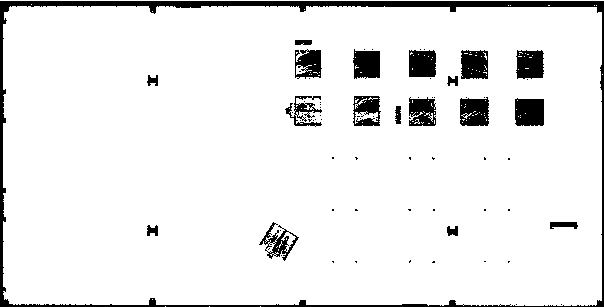
\includegraphics[width=\textwidth]{./figures/depot.png}
    \caption{Depot. Dimensions: 30.2 m by 15.3 m.}
  \end{subfigure}
  \hfill
  \begin{subfigure}[b]{0.46\textwidth}
    \centering
    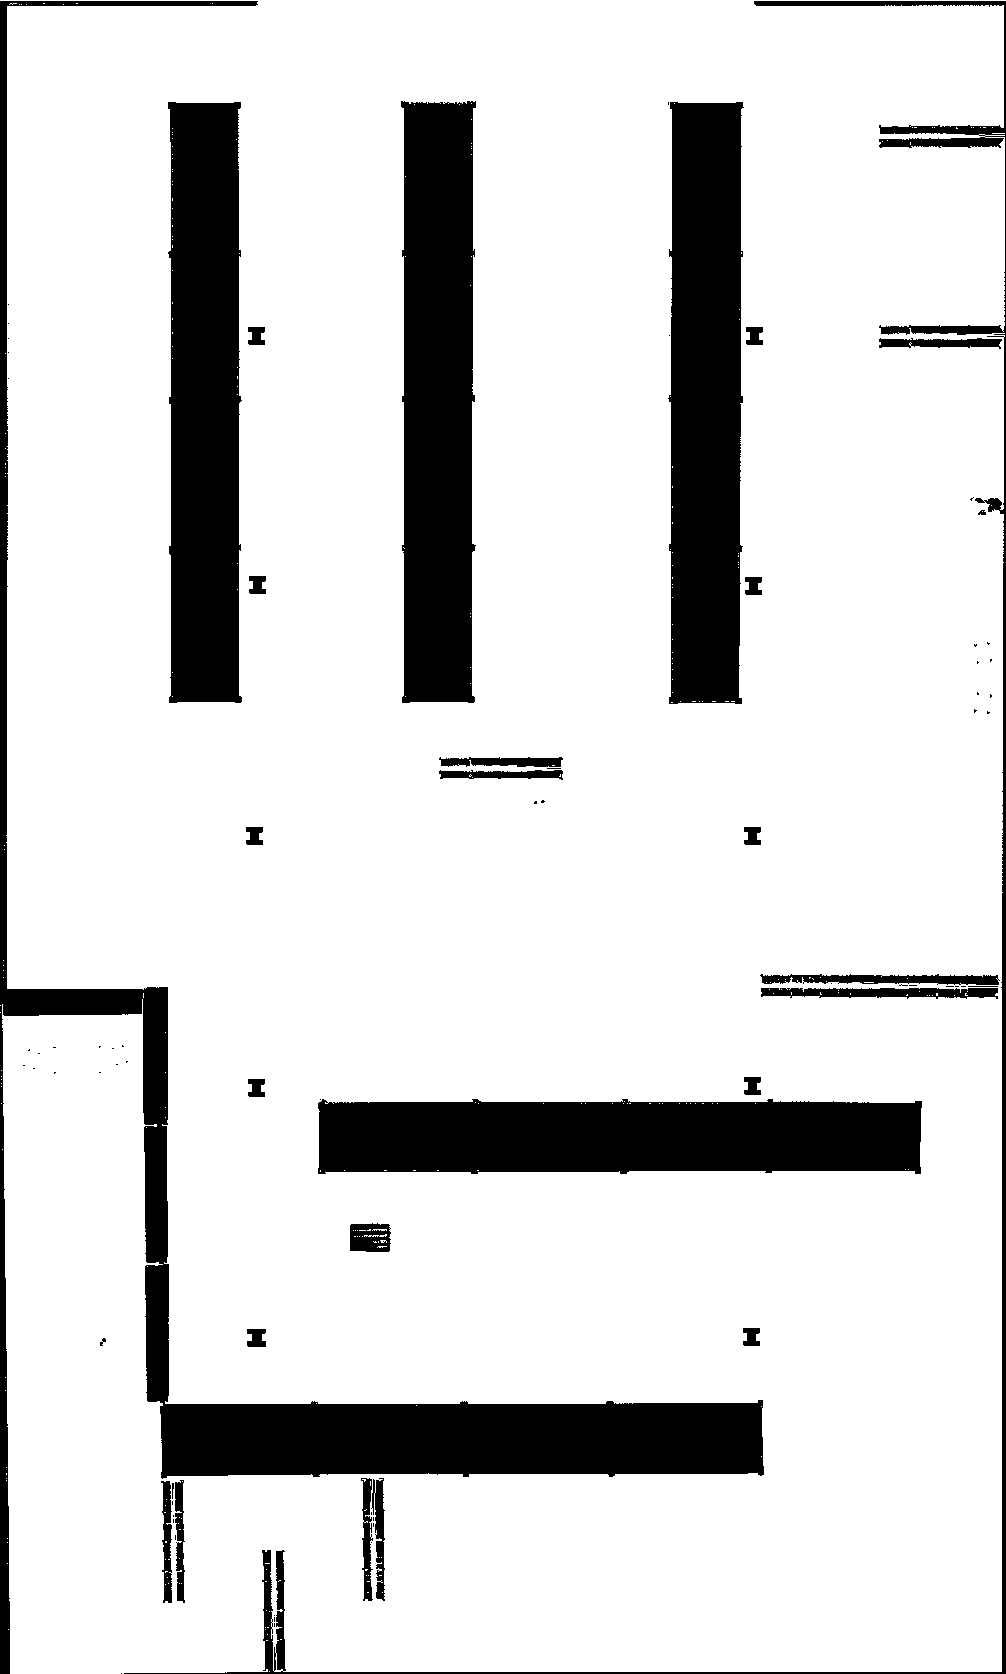
\includegraphics[height=\textwidth, angle=90]{./figures/warehouse.png}
    \caption{Warehouse. Dimmensions: 50.2 m by 30.2 m.}
  \end{subfigure}
  \caption{Maps used for benchmarking search algorithms. The Depot map is smaller and more open compared to the Warehouse map, which is larger and has more hard to reach areas.}
  \label{fig:bench-maps}
\end{figure}

\subsection{Botplot}
To enable efficient and reproducible experimentation, a custom Python package named \texttt{botplot} was developed. This tool provides utility functions for running and analyzing scenarios in both \texttt{simple\_sim} and the Gazebo/ROS 2 simulation environments.

During each simulation run, data is collected in real time. In \texttt{simple\_sim}, the data is recorded directly and stored in a \texttt{.ipc} (Apache Arrow) file. Similarly, in the ROS 2 setup, a dedicated logger node captures relevant simulation data, which is likewise serialized for later analysis.\\

Once recorded, the data is processed using \texttt{botplot}, which offers a suite of customizable plotting functions to visualize various performance metrics. These include map coverage, robot paths, communication patterns, and computational performance, among others.

To streamline the workflow, results are cached based on the simulation scenario. This allows for rapid re-plotting without the need to rerun the simulation, significantly improving the iteration speed when tuning parameters or updating visualizations.

All figures presented in this report were generated using \texttt{botplot}.

\subsection{Simulator Consistency}
\label{sec:simulator-consistency}
A central goal of the dual-simulator setup is to ensure that algorithms implemented using the \texttt{botbrain} interface yield consistent behavior across both simulators. While Gazebo includes more realistic physics and non-deterministic behavior due to its time step and sensor noise, consistency in qualitative behavior (e.g., coverage trend) is still expected.

\subsubsection{Movement Calibration}
To verify basic motion consistency, simple movement behaviors were executed in both simulators. Speed and steer commands were scaled to get the paths shown in \cref{fig:movement-consistency}. 

\begin{figure}[H]
  \centering
  \begin{subfigure}[b]{0.45\textwidth}
    \centering
    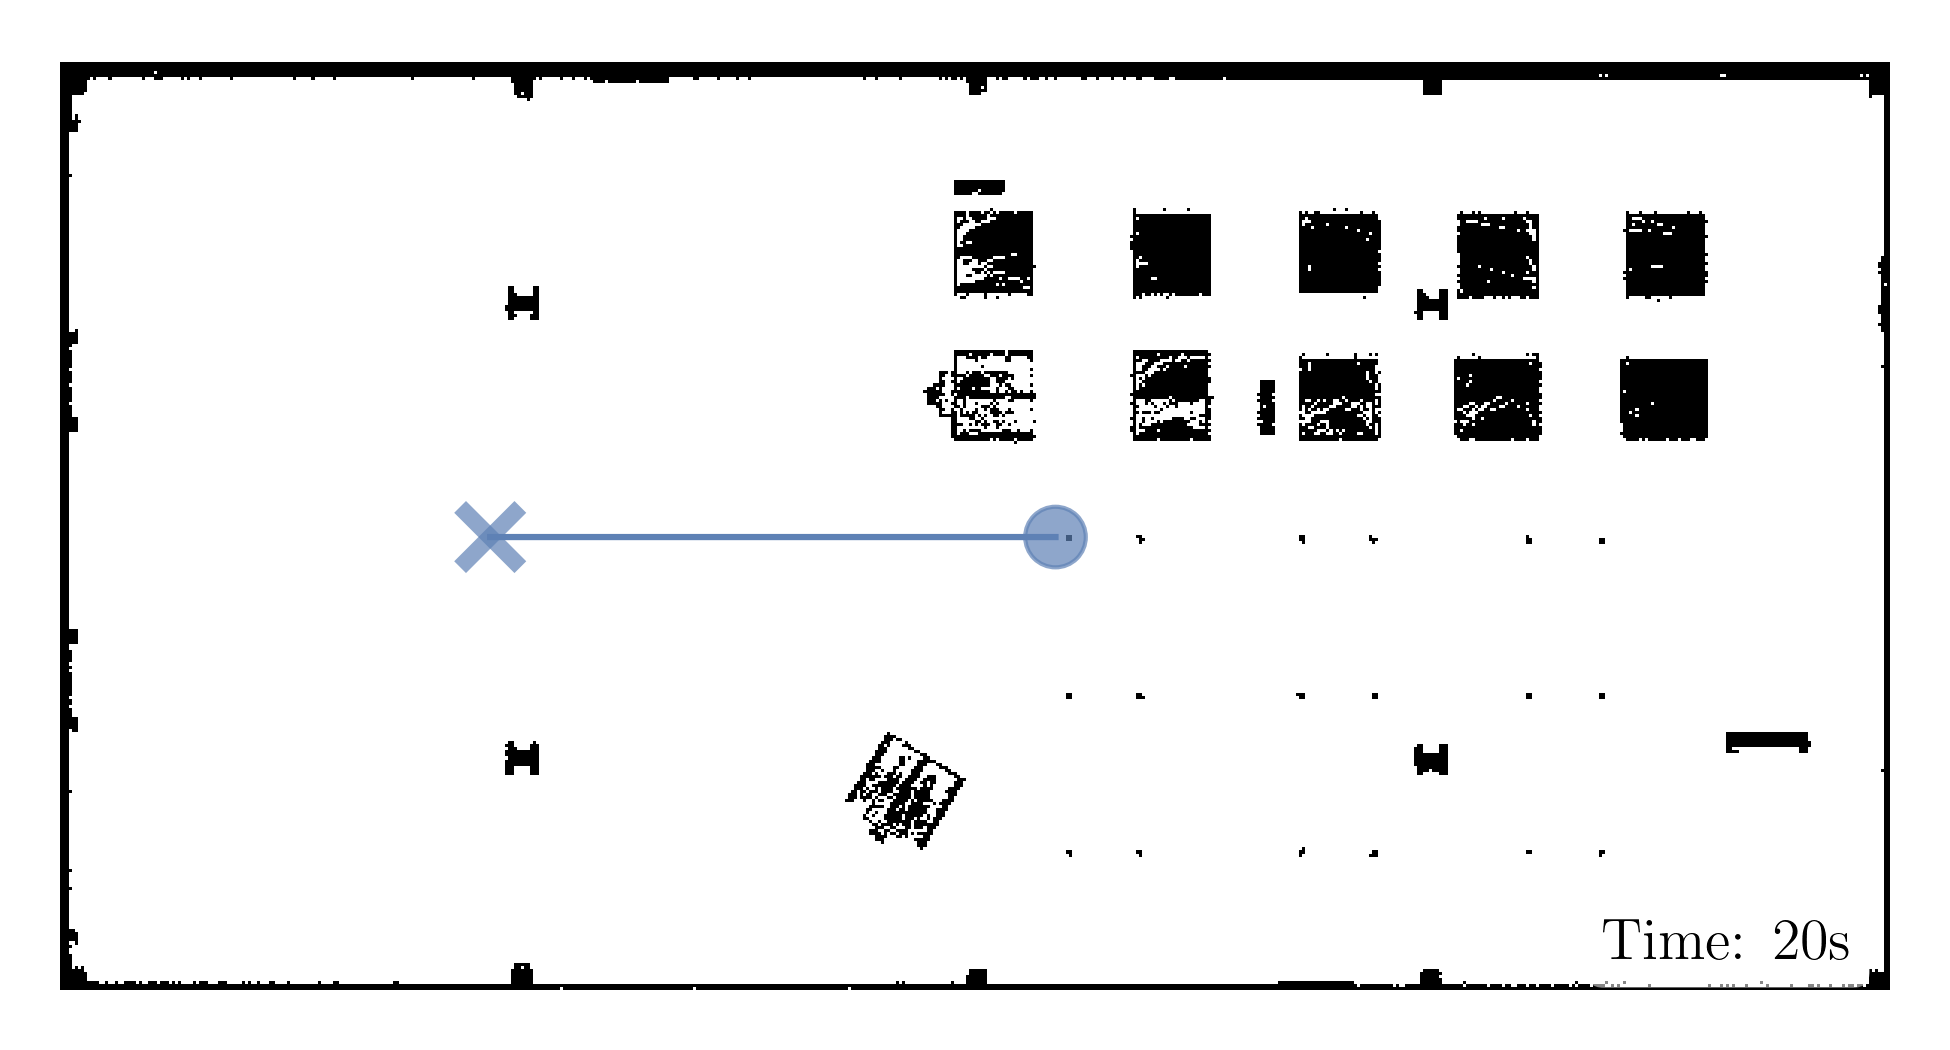
\includegraphics[width=\textwidth]{./figures/plots/consistency/simple-sim-paths-straight.png}
    \caption{\texttt{simple\_sim} straight line.}
  \end{subfigure}
  \begin{subfigure}[b]{0.45\textwidth}
    \centering
    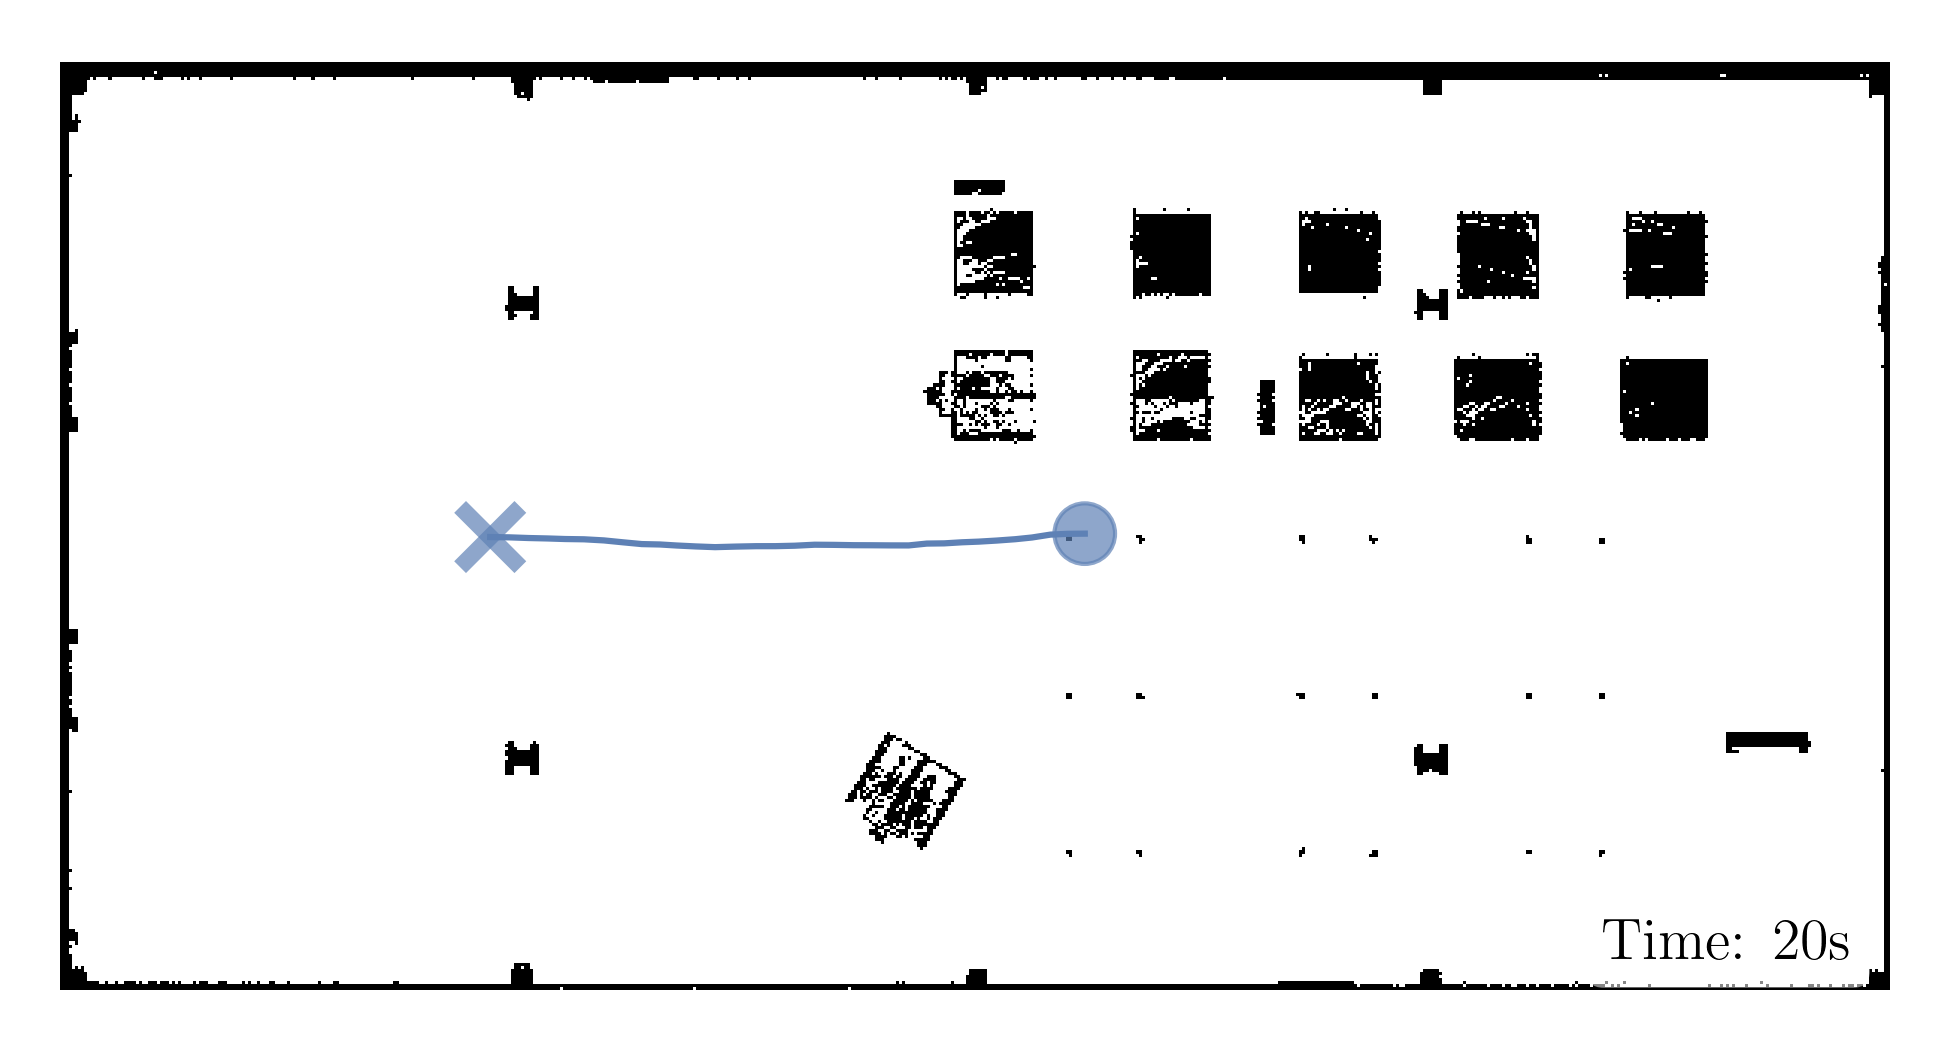
\includegraphics[width=\textwidth]{./figures/plots/consistency/ros-2-paths-straight.png}
    \caption{ROS 2 Gazebo straight line.}
  \end{subfigure}\\
  \begin{subfigure}[b]{0.45\textwidth}
    \centering
    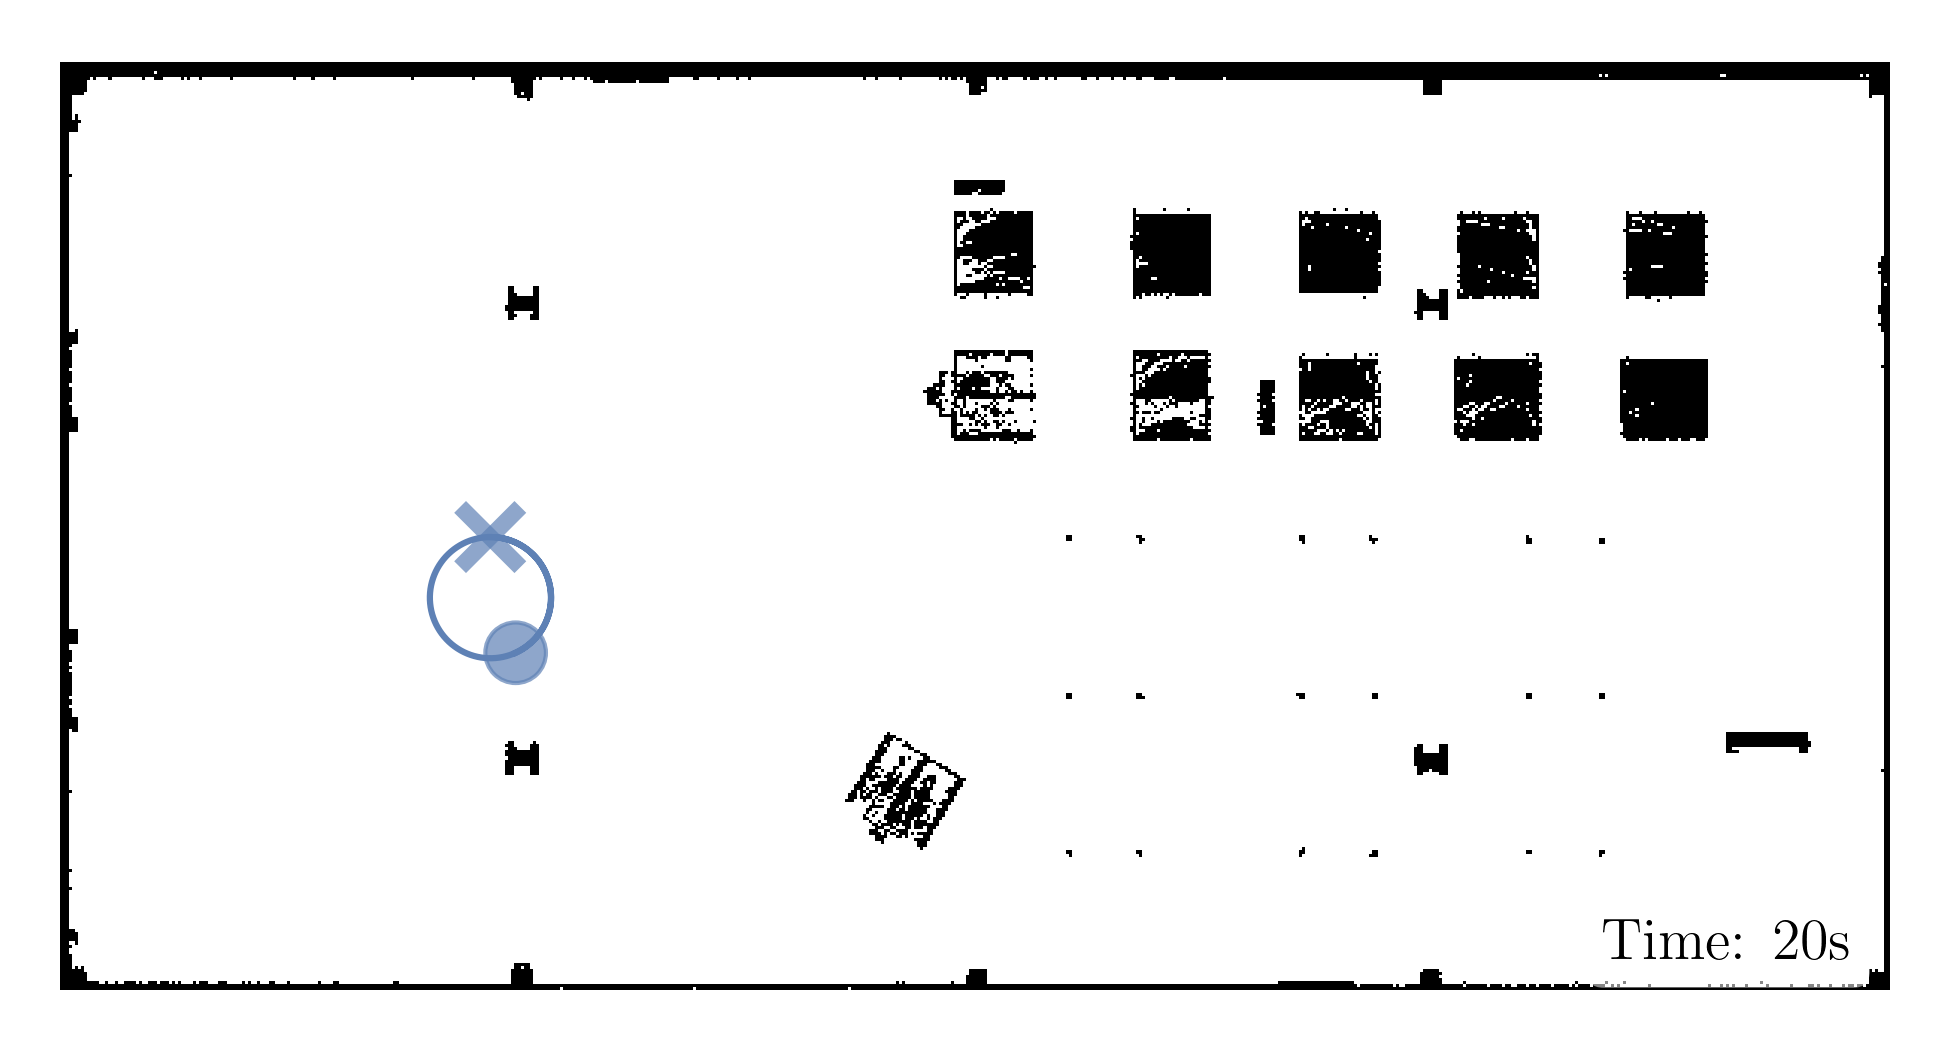
\includegraphics[width=\textwidth]{./figures/plots/consistency/simple-sim-paths-circle.png}
    \caption{\texttt{simple\_sim} circular.}
  \end{subfigure}
  \begin{subfigure}[b]{0.45\textwidth}
    \centering
    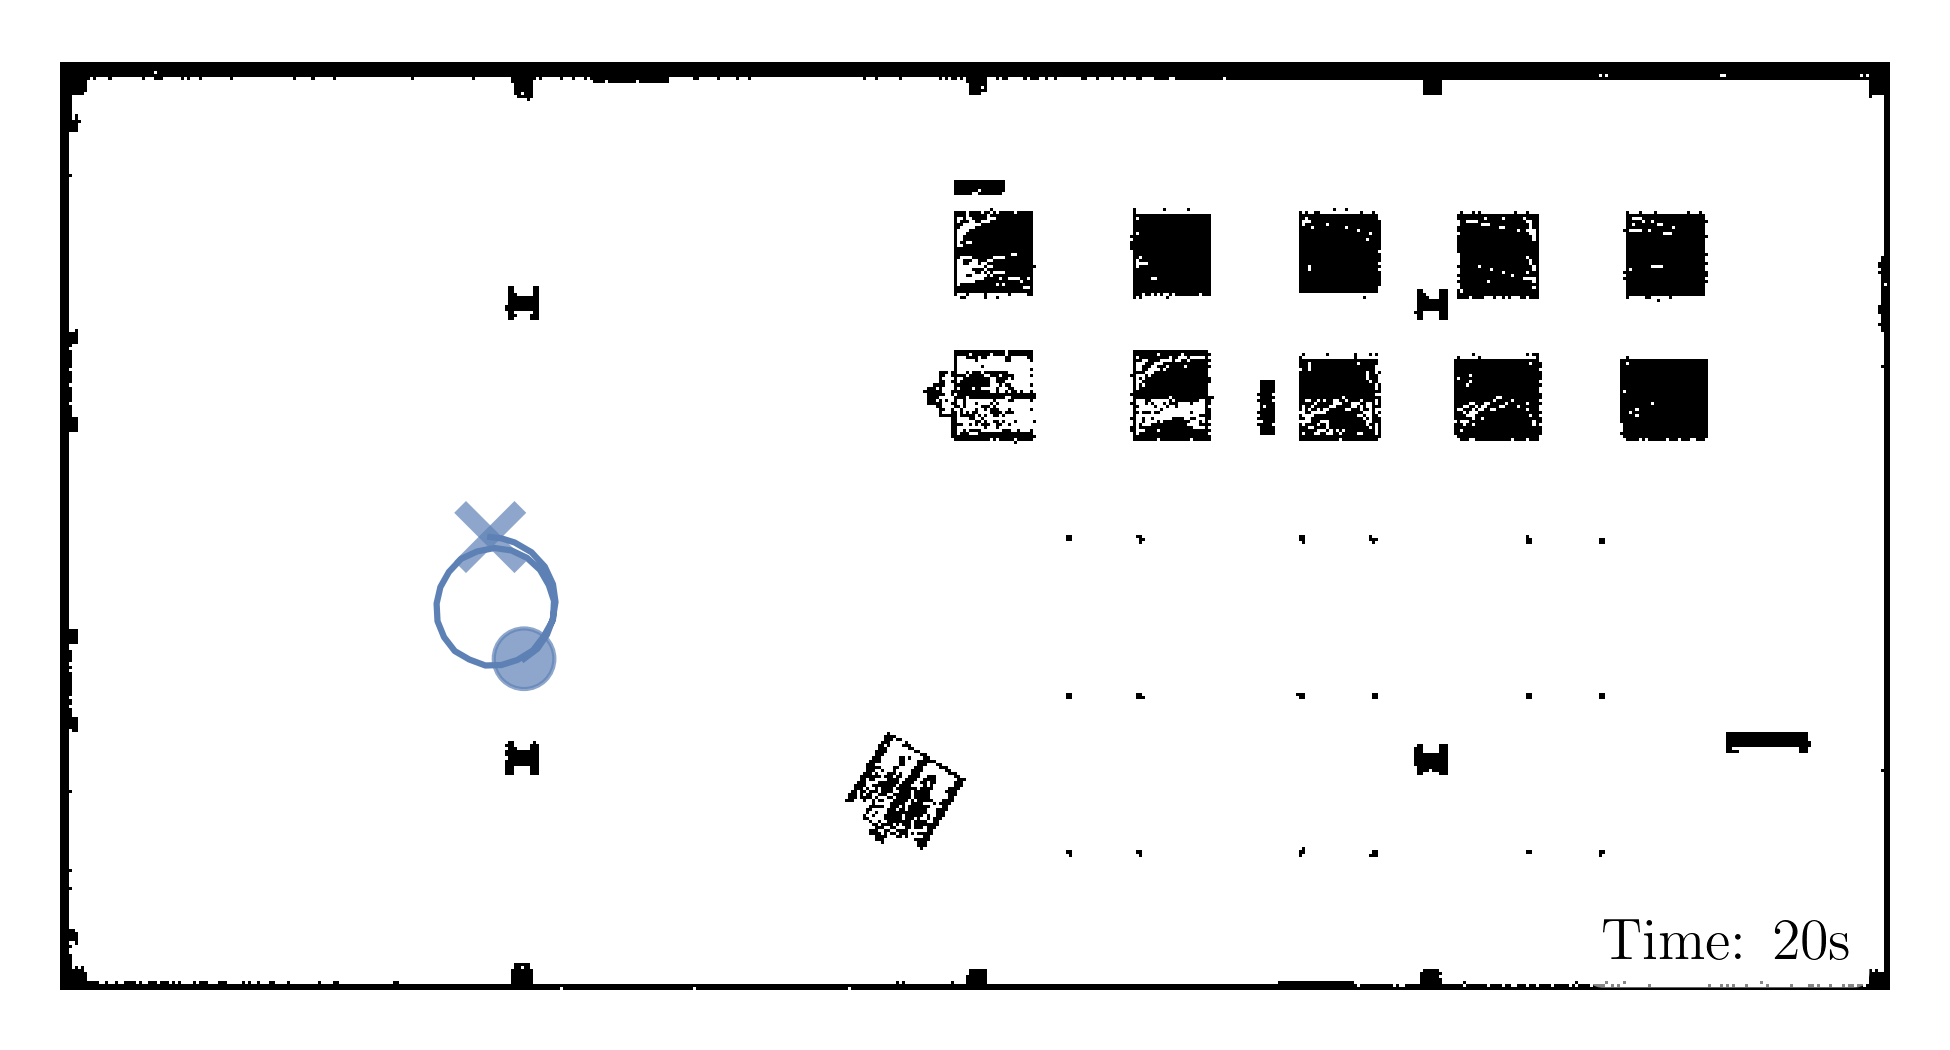
\includegraphics[width=\textwidth]{./figures/plots/consistency/ros-2-paths-circle.png}
    \caption{ROS 2 Gazebo circular.}
  \end{subfigure}
  \caption{Paths produced by \texttt{simple\_sim} and ROS 2 Gazebo.}
  \label{fig:movement-consistency}
\end{figure}

The paths are visually similar, indicating that the velocity commands generated by the behavior logic are interpreted consistently across both environments.

\subsubsection{Performance Consistency}
To validate performance characteristics across simulators, the coverage of 4 robots was recorded over 6 runs for the behaviors developed in \cref{sec:search-algorithms} in both simulators. \Cref{fig:coverage-benchmark-all} shows the results of this test.

\begin{figure}[H]
    \centering
    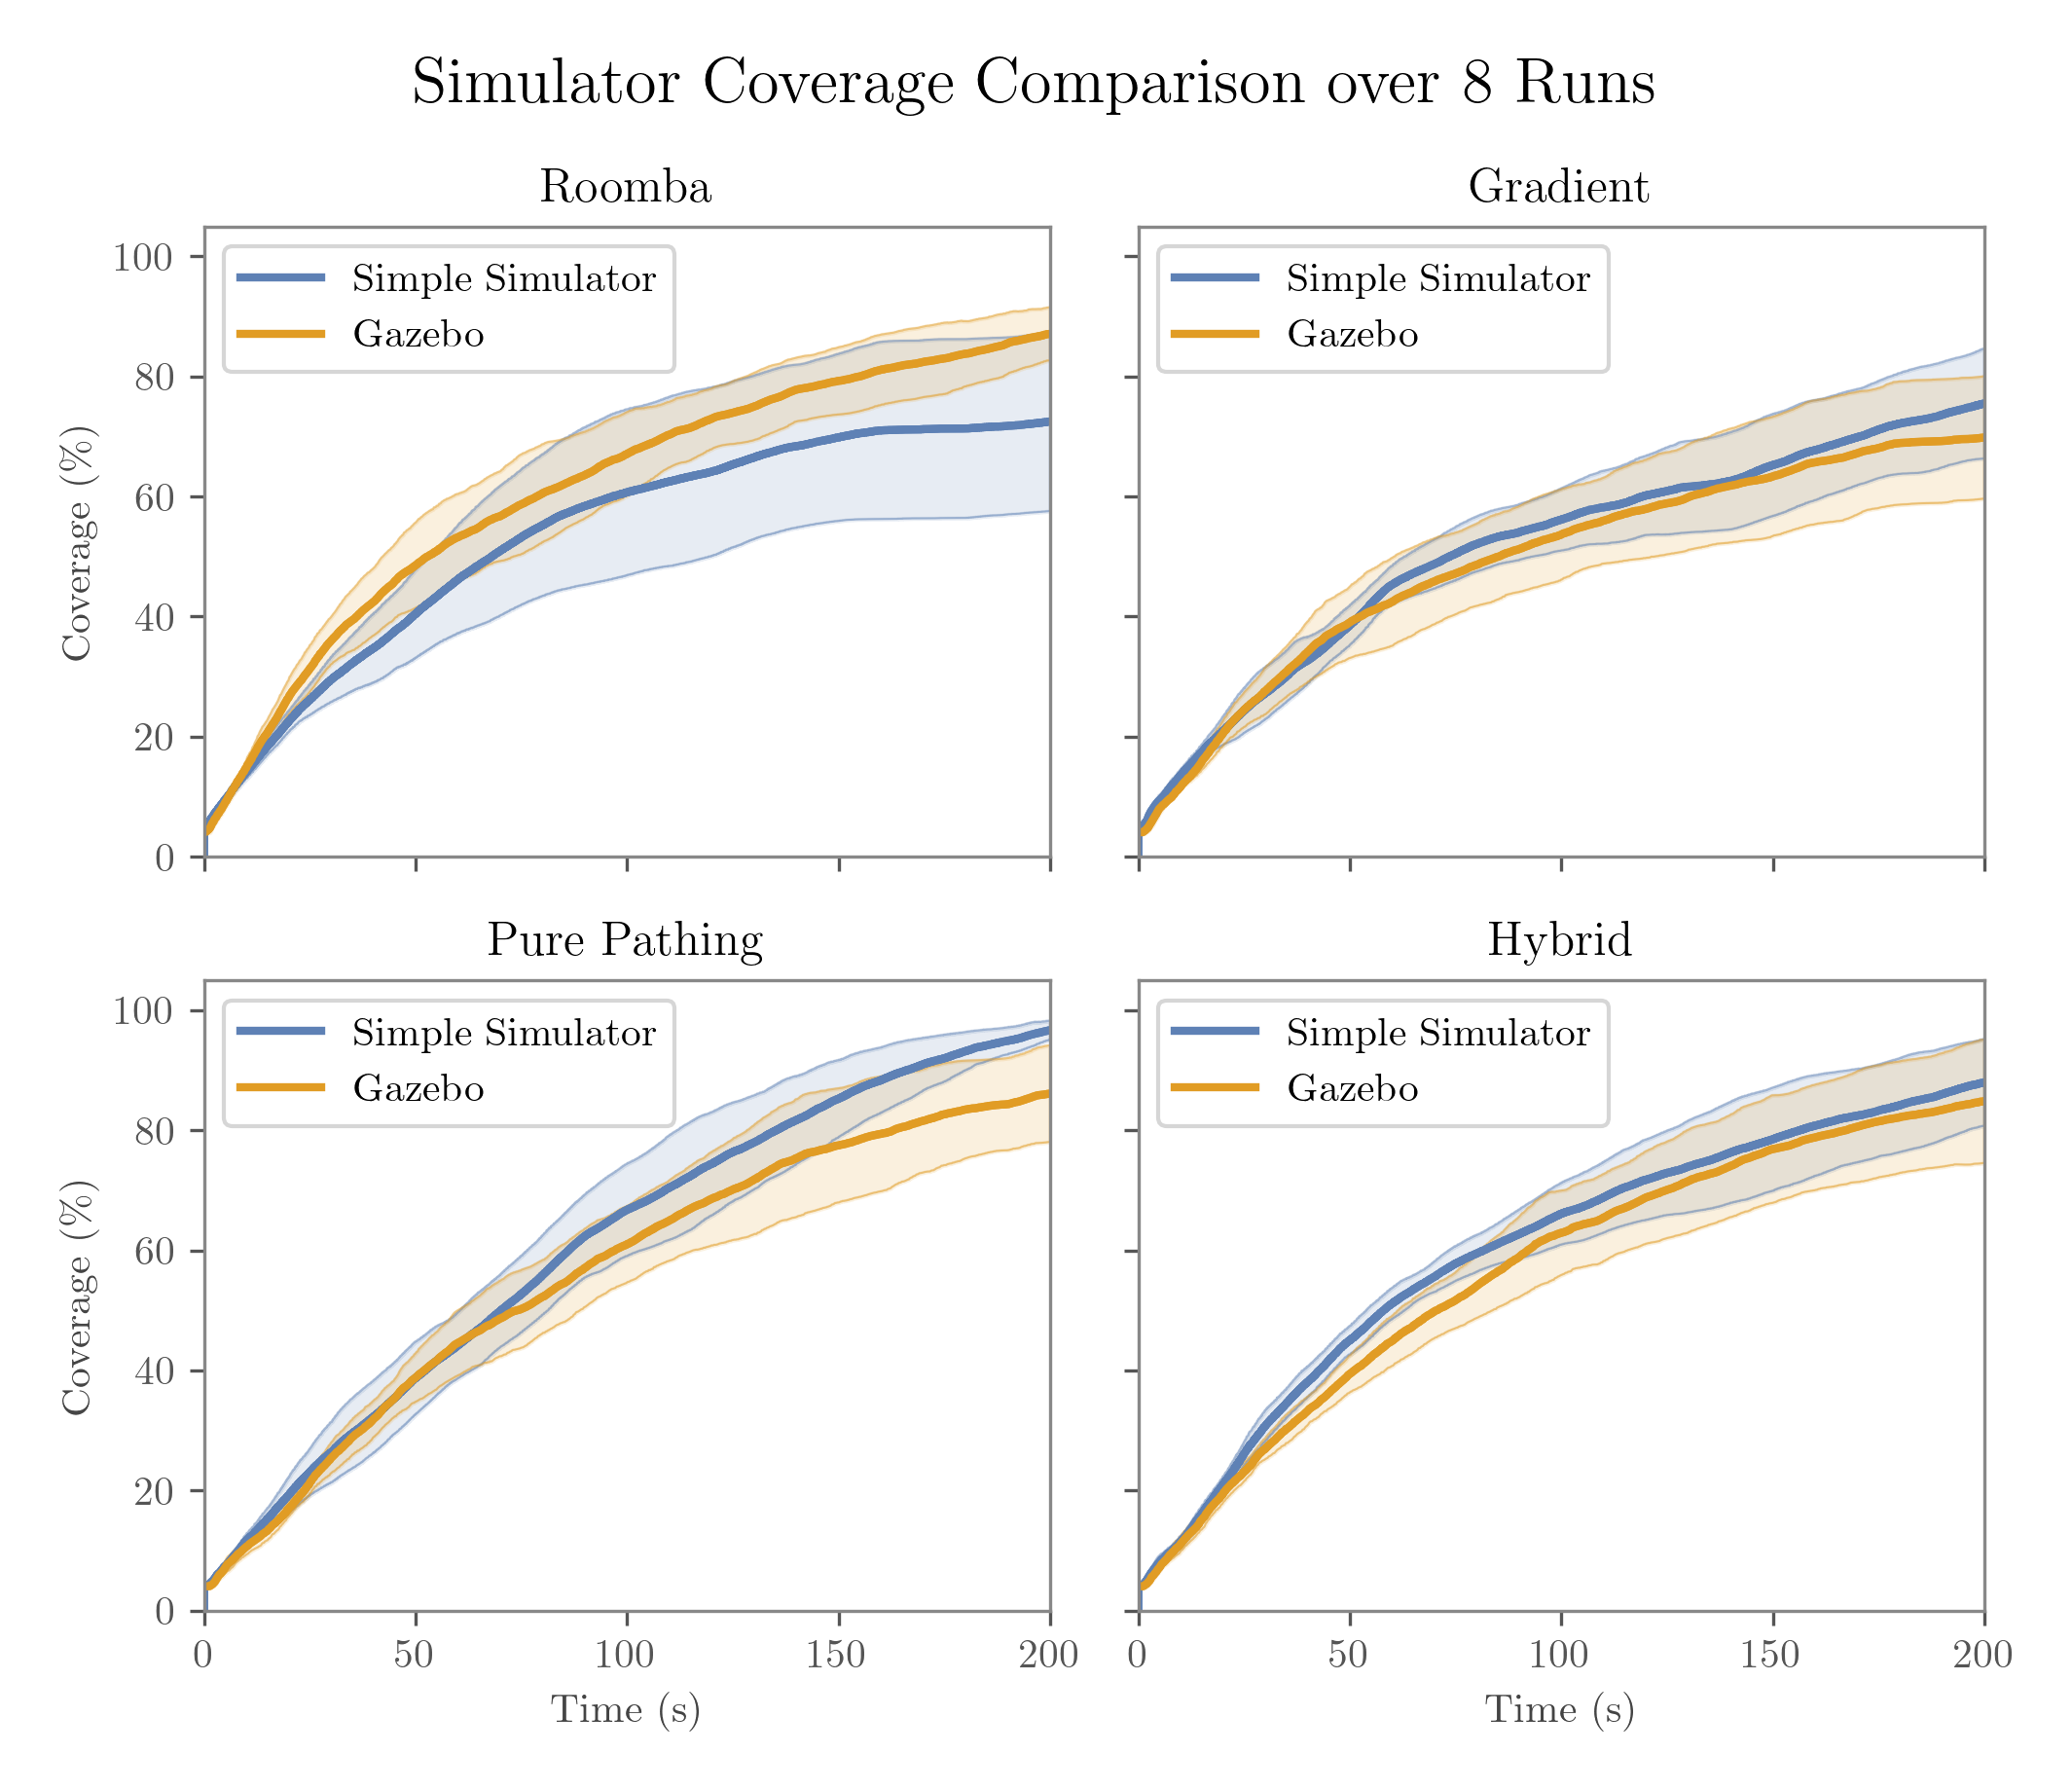
\includegraphics[width=0.95\textwidth]{./figures/plots/consistency/gazebo_vs_simple_sim_coverage.png}
    \caption{Comparison of coverage over time between ROS 2 Gazebo and \texttt{simple\_sim}.}
    \label{fig:coverage-benchmark-all}
\end{figure}

The coverage performance seems to match well between the two simulators, with coverage mostly staying within 1 standard deviation of each other. The Roomba algorithm does, however, seem to perform better in the gazebo environment. \Cref{fig:coverage-benchmark-diff} shows the difference in coverage performance.

\begin{figure}[H]
    \begin{center}
        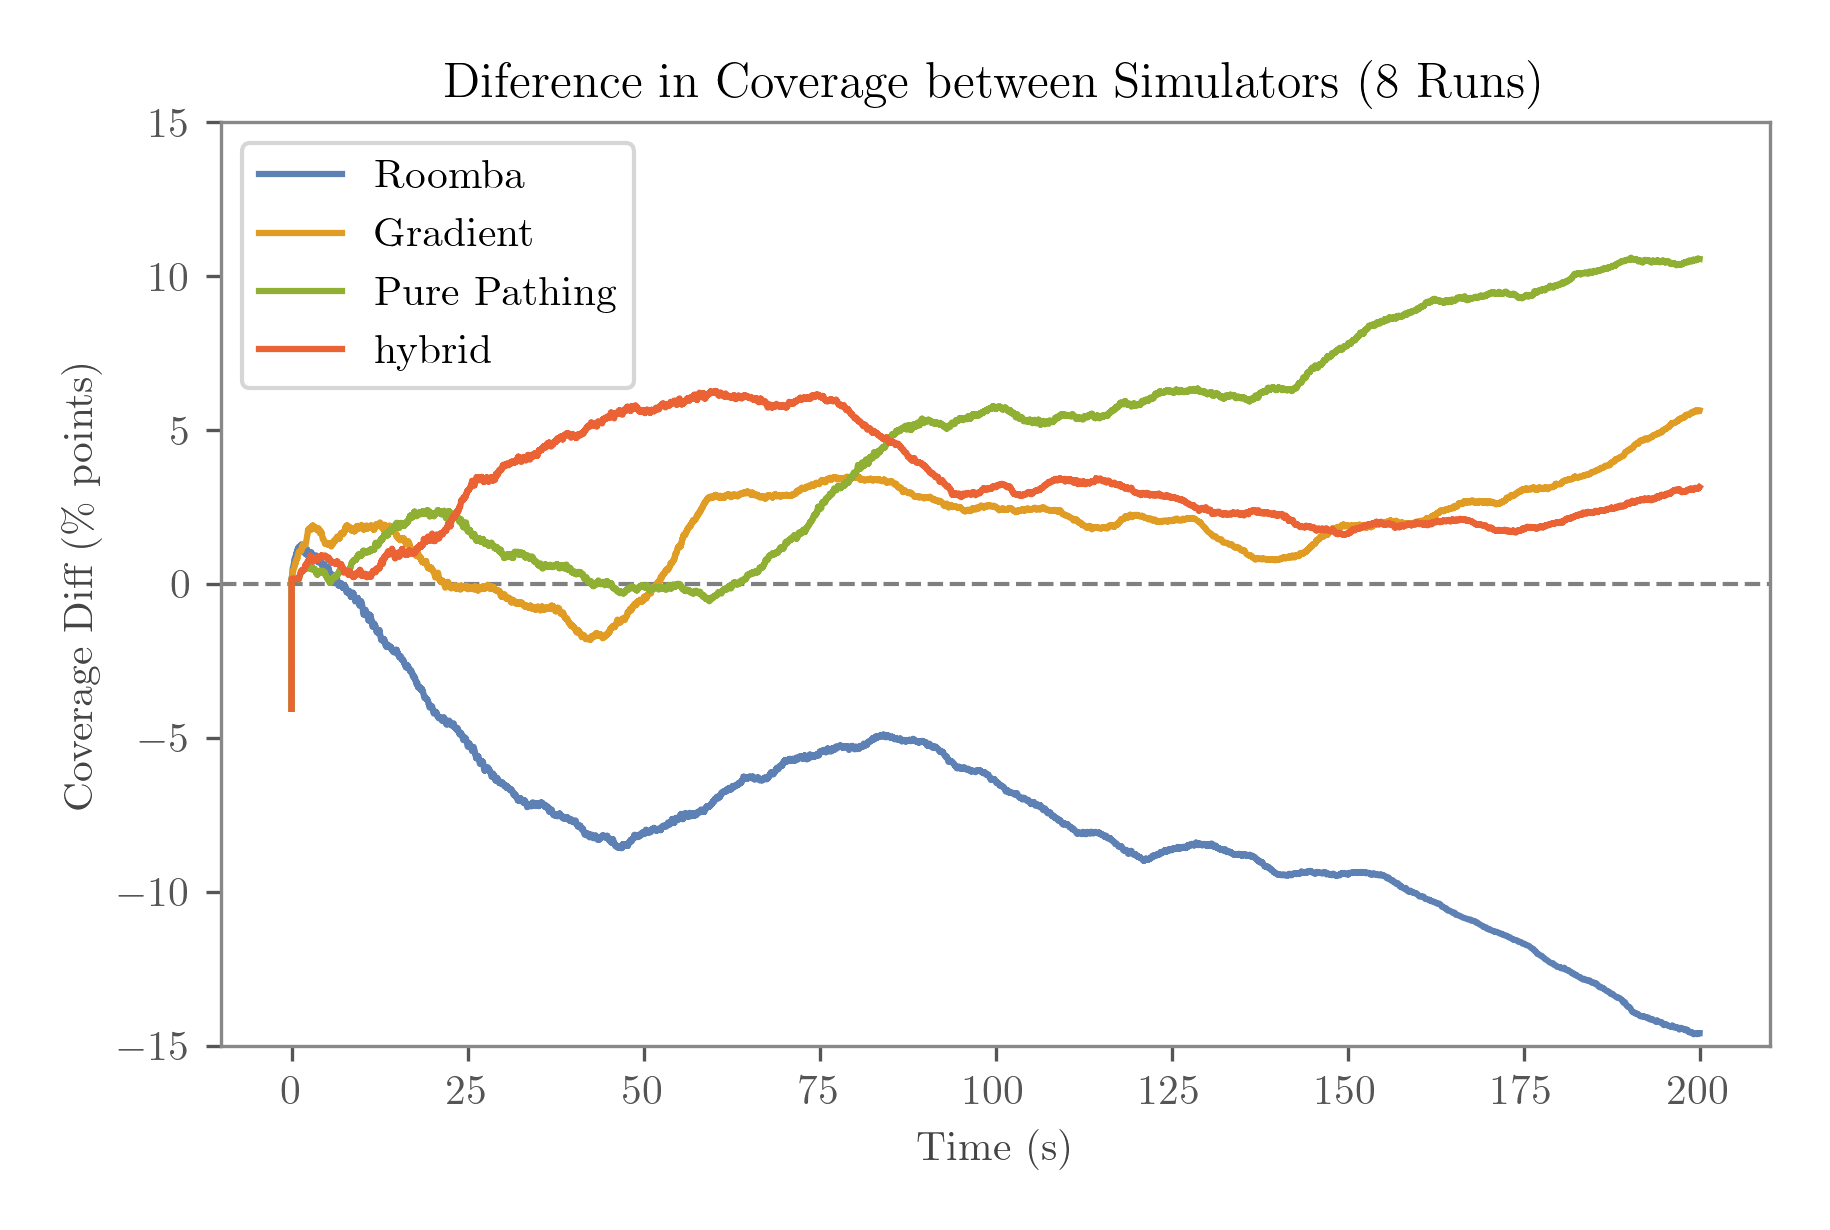
\includegraphics[width=0.90\textwidth]{./figures/plots/consistency/sim_coverage_diff.png}
    \end{center}
    \caption{Comparison of difference in coverage over time between ROS 2 Gazebo and \texttt{simple\_sim}.}
    \label{fig:coverage-benchmark-diff}
\end{figure}

\subsection{Search Algorithm Benchmarks}
\label{sec:search-algorithms-benchmark}
Each algorithm was run 10 times on the Depot (for 800 s) and Warehouse (for 1200 s) maps with 1, 2, 4, 8 robots using \texttt{simple\_sim}. The warehouse map was also run with 16 robots. The relative performance between the behaviors seems stable regardless of robot count. \Cref{fig:coverage-benchmark} shows a representative result with 4 robots. All results can be found in Appendix \ref{appendix:more-plots}. 

\begin{figure}[H]
  \centering
  \begin{subfigure}[b]{0.49\textwidth}
    \centering
    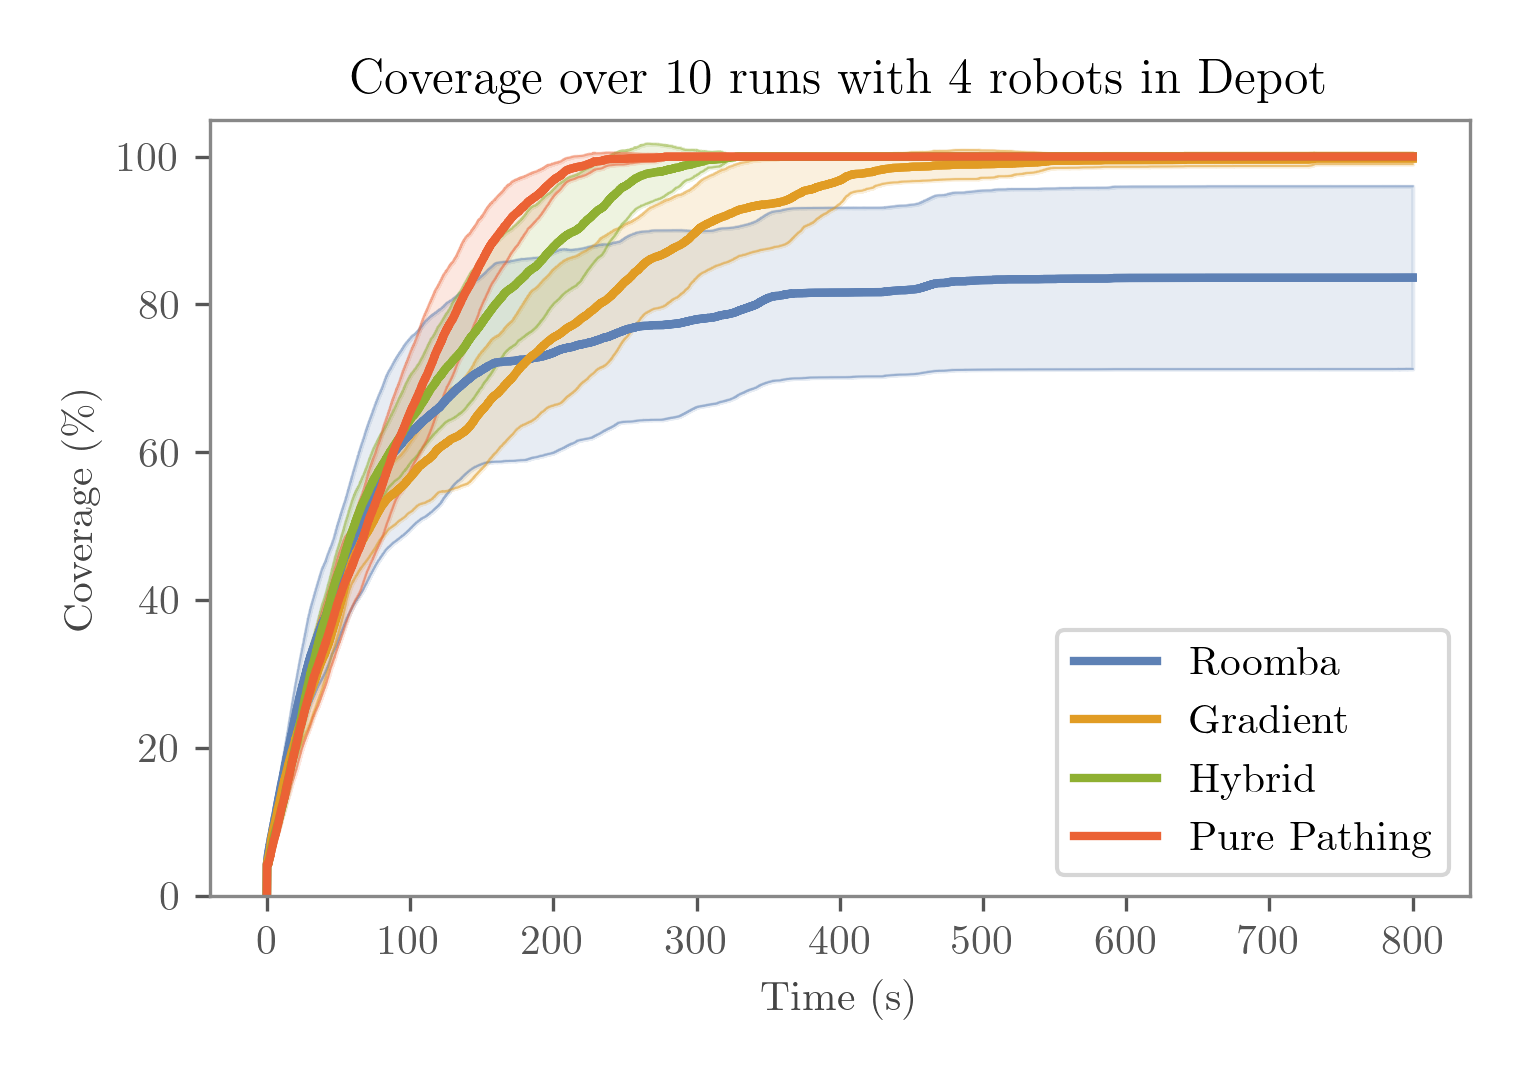
\includegraphics[width=\textwidth]{./figures/plots/benchmarks/coverage-over-10-runs-with-4-robots-in-depot.png}
      \caption{800 s in simple map (Depot)}
  \end{subfigure}
  \begin{subfigure}[b]{0.49\textwidth}
    \centering
    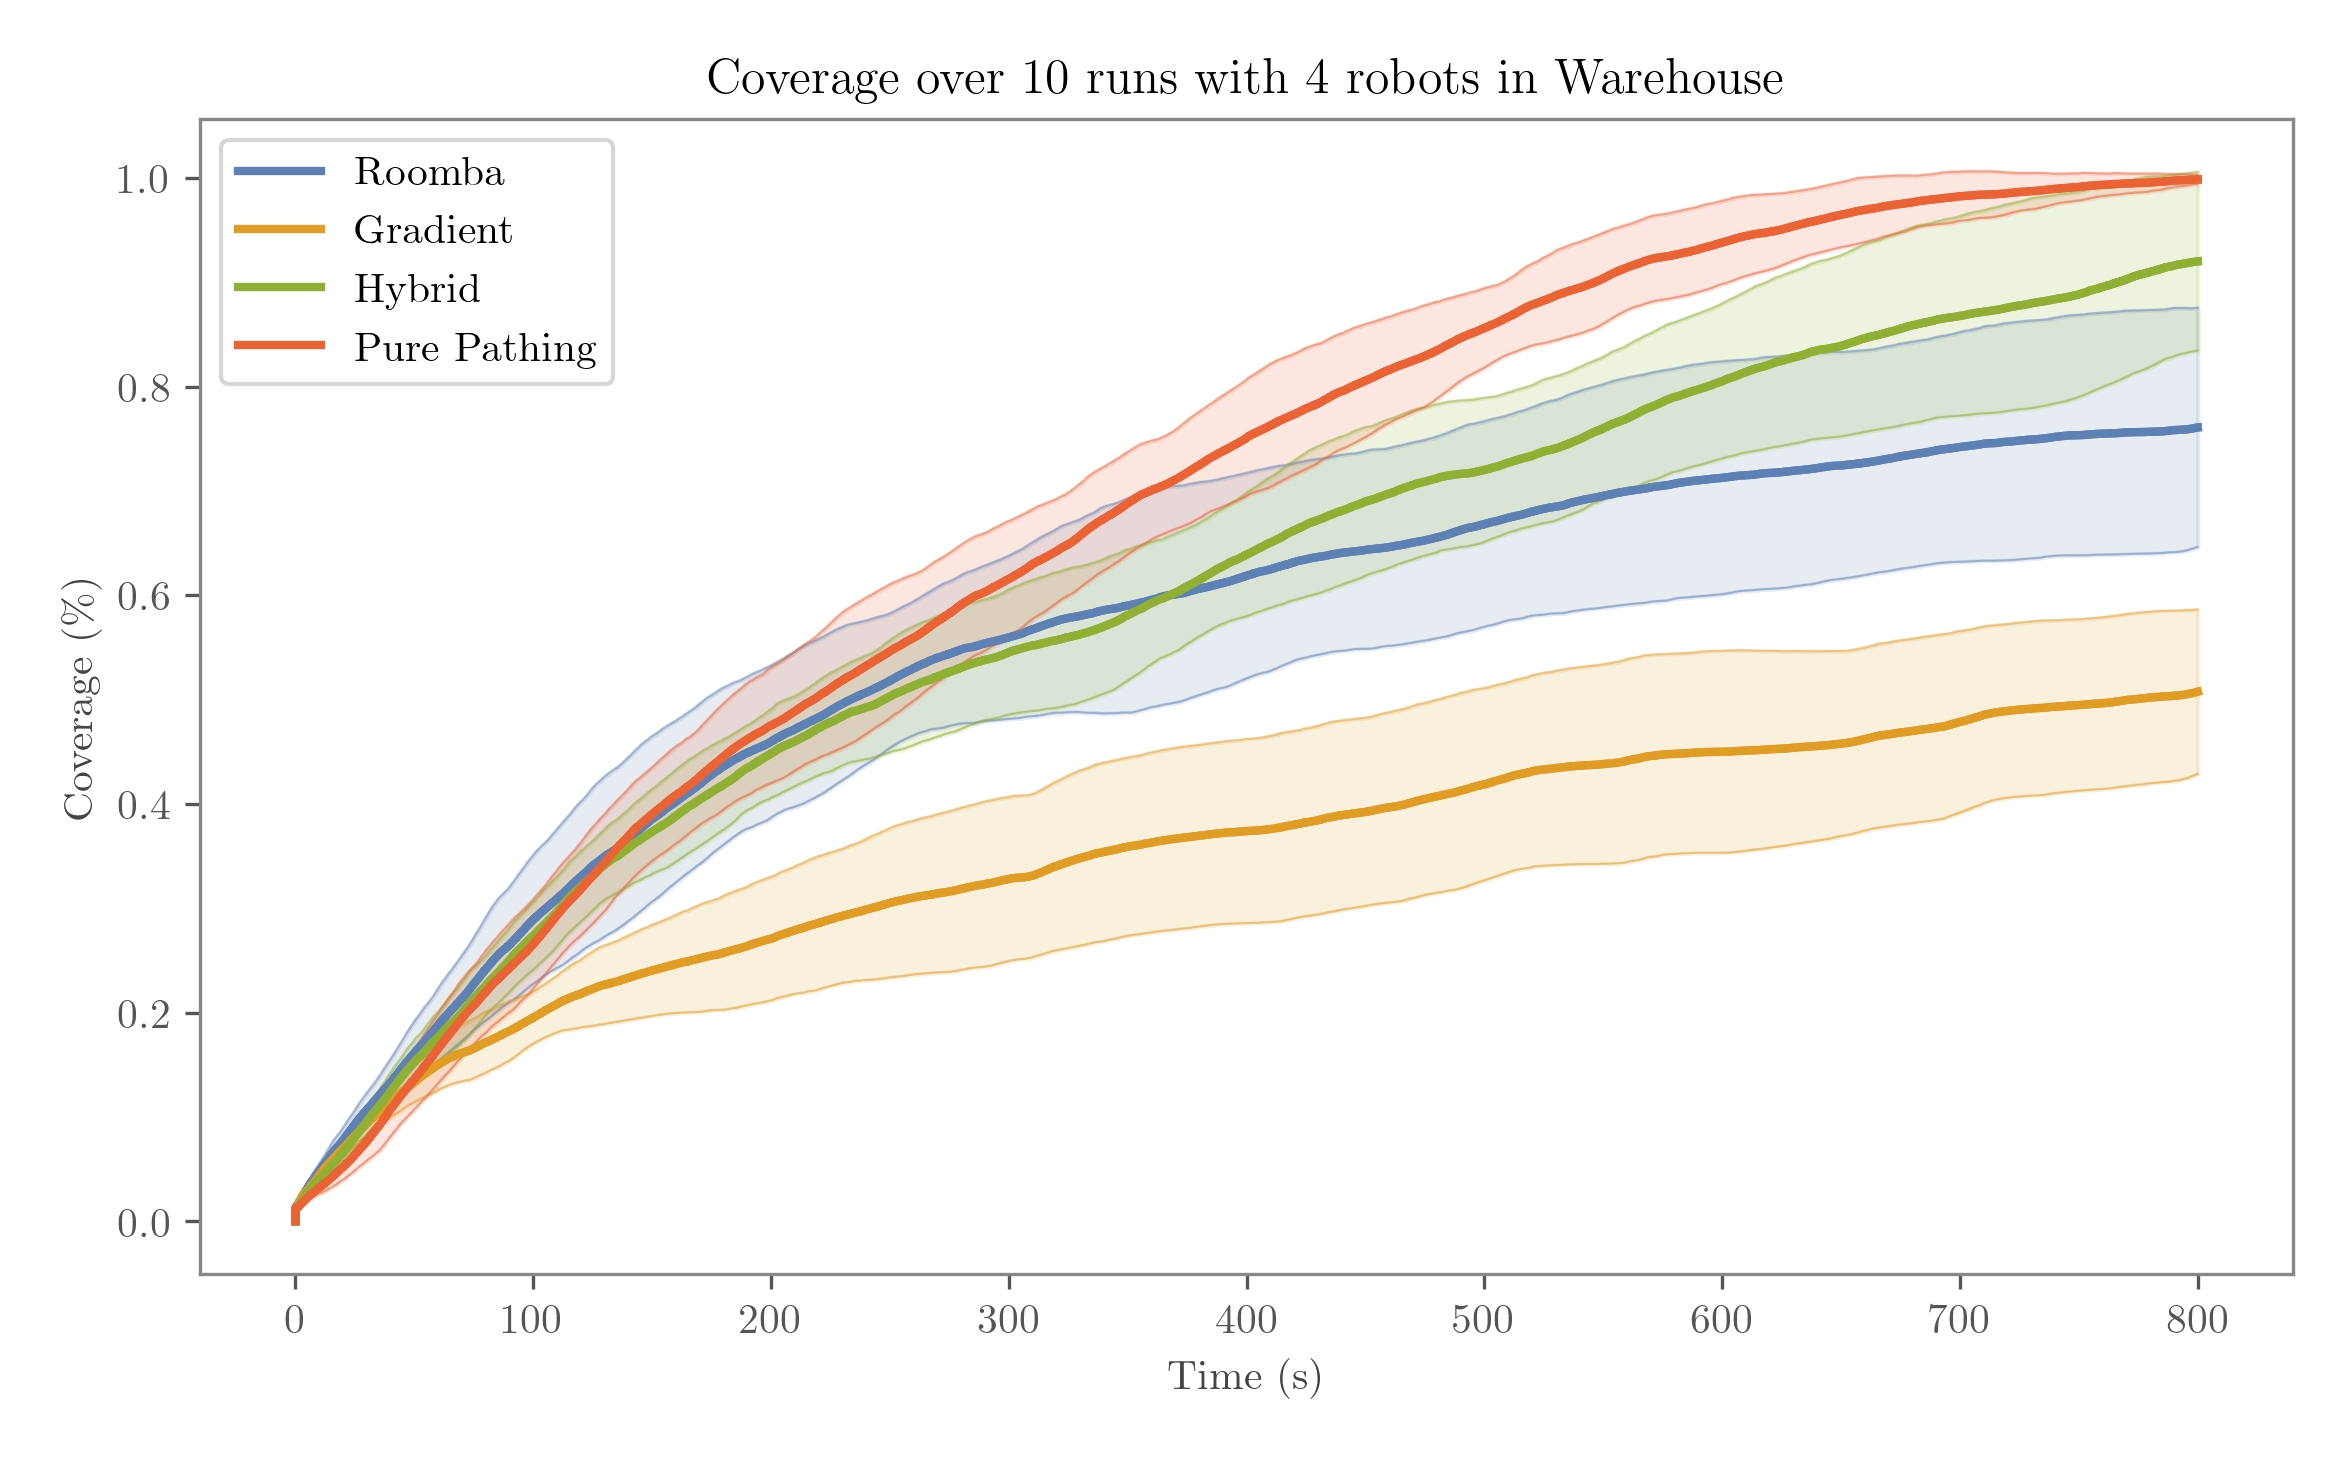
\includegraphics[width=\textwidth]{./figures/plots/benchmarks/coverage-over-10-runs-with-4-robots-in-warehouse.png}
      \caption{1200 s in complex map (Warehouse)}
  \end{subfigure}
    \caption{Coverage performance of search algorithms over 10 runs with 4 robots starting in random positions in the same environment.}
    \label{fig:coverage-benchmark}
\end{figure}

The results clearly show that the Pure Pathing outperforms the other algorithms followed by the Hybrid algorithm. The Gradient algorithm is significantly worse than both the Pure Pathing and Hybrid algorithms. The Roomba algorithm is generally better performing in the beginning of the run, but has a hard time getting full coverage of the map, and is overtaken by the Gradient algorithm which has the search gradient to guide it towards unexplored areas.

\def\w{0.329\textwidth}
\begin{figure}[H]
    \centering
    \begin{subfigure}[b]{\w}
        \centering
        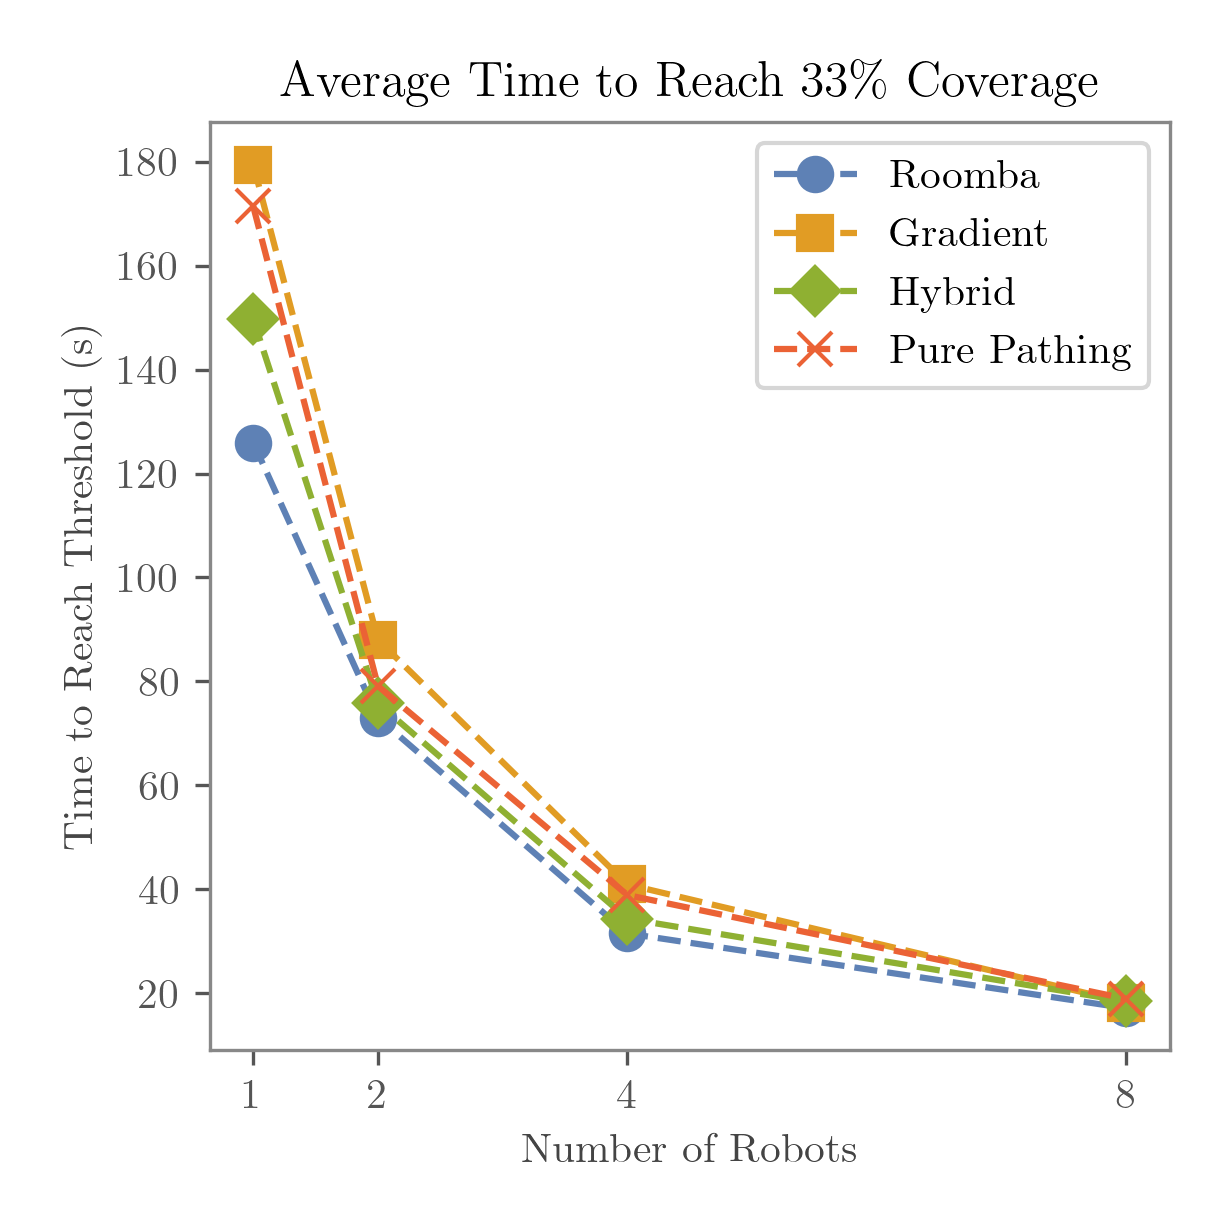
\includegraphics[width=\textwidth]{figures/plots/benchmarks/big-coverage-0.33-depot.png}
    \end{subfigure}
    \begin{subfigure}[b]{\w}
        \centering
        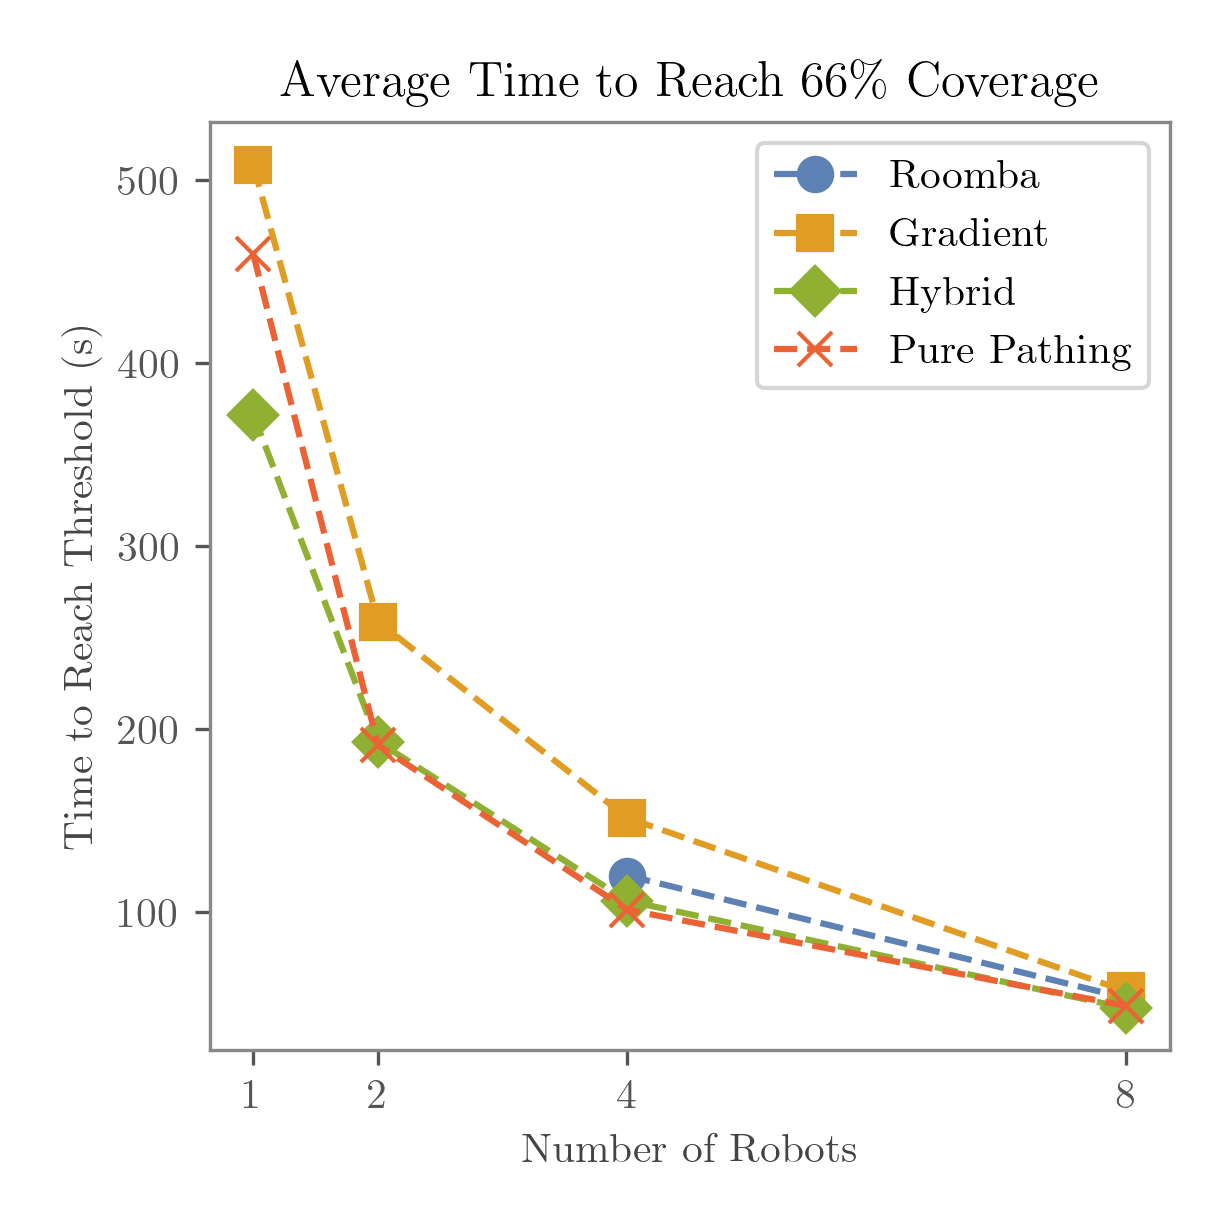
\includegraphics[width=\textwidth]{figures/plots/benchmarks/big-coverage-0.66-depot.png}
    \end{subfigure}
    \begin{subfigure}[b]{\w}
        \centering
        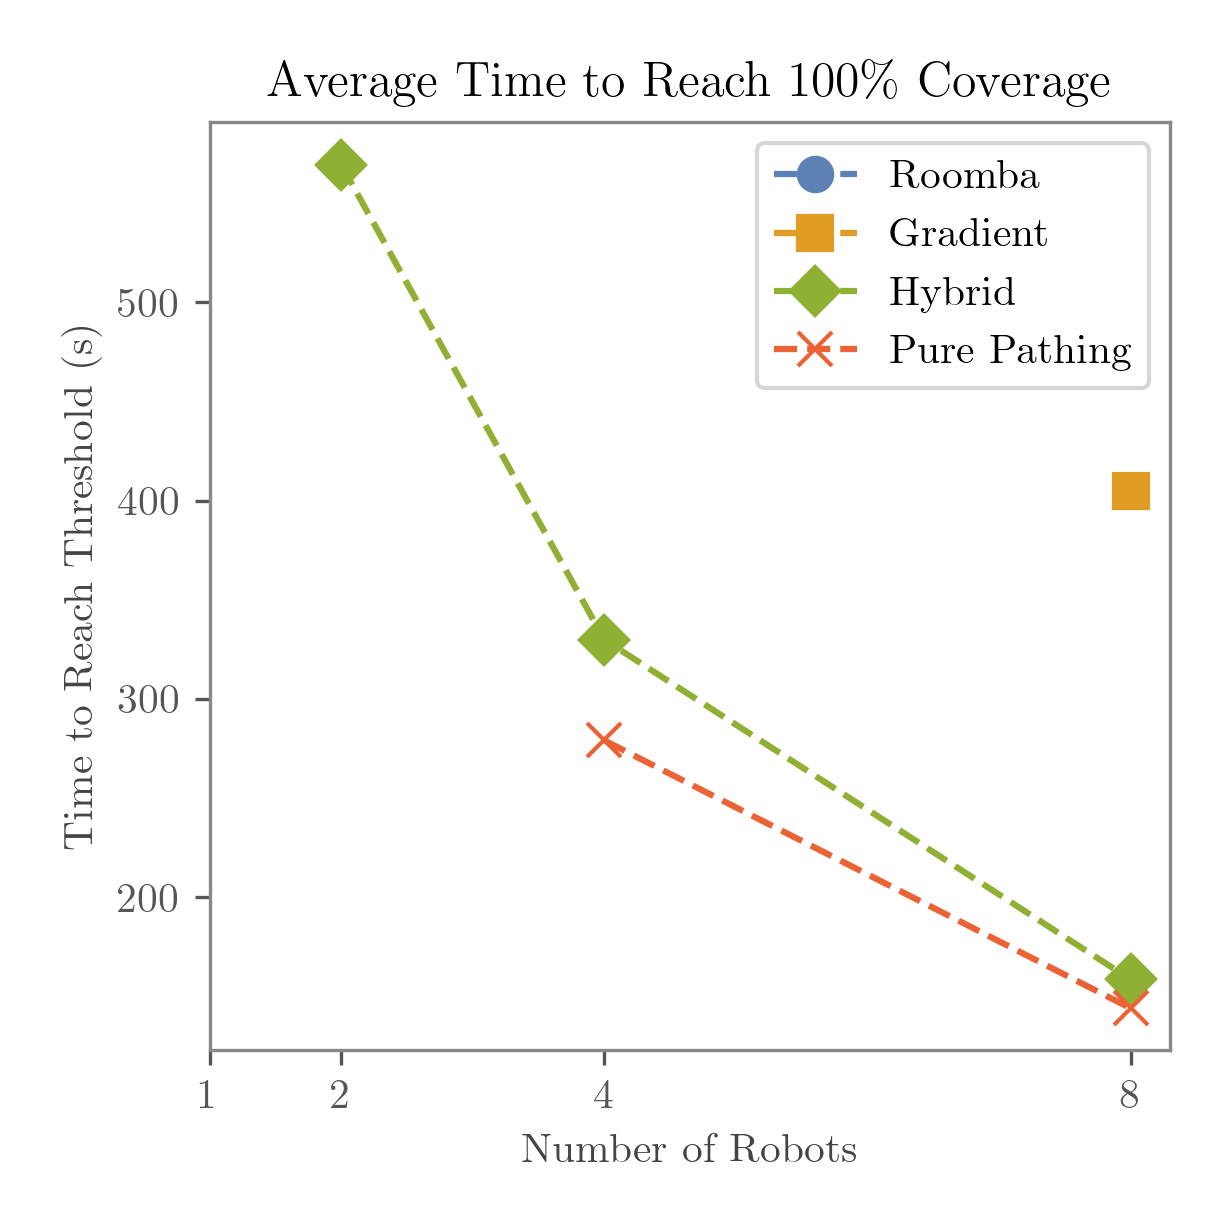
\includegraphics[width=\textwidth]{figures/plots/benchmarks/big-coverage-1.0-depot.png}
    \end{subfigure}
    \caption{Average time it takes the swarm to cover 33\%, 66\% and 100\% of the map in the Depot environment over 10 runs. Points are left out if the swarm did not reach these thresholds on average.}
    \label{fig:depot-threshold}
\end{figure}

\def\w{0.329\textwidth}
\begin{figure}[H]
    \centering
    \begin{subfigure}[b]{\w}
        \centering
        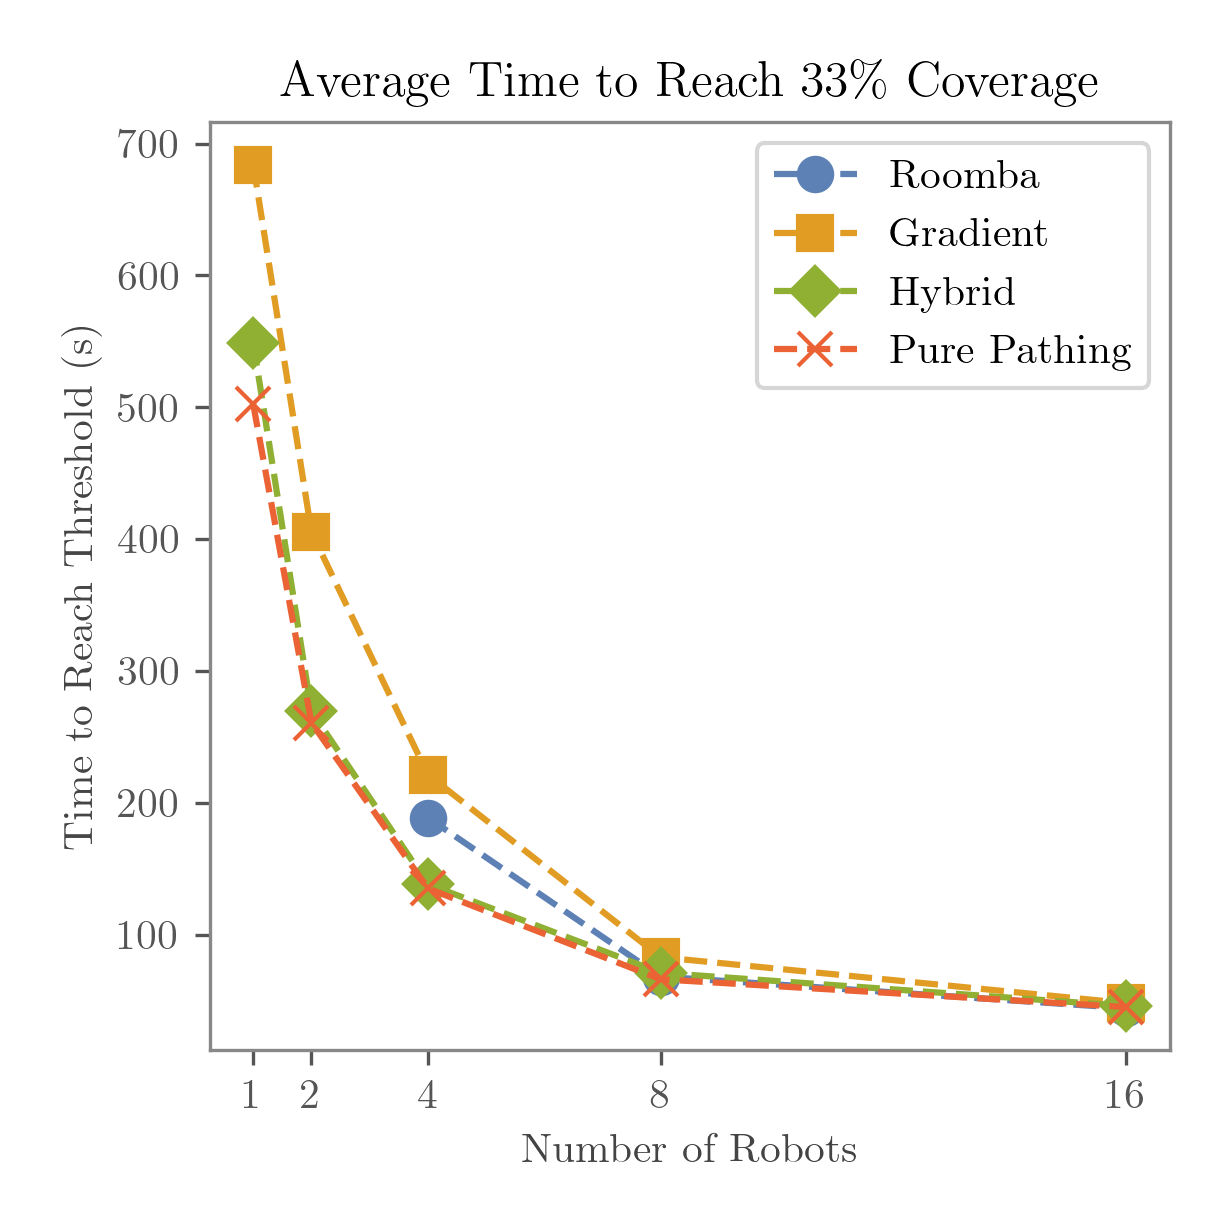
\includegraphics[width=\textwidth]{figures/plots/benchmarks/big-coverage-0.33-warehouse.png}
    \end{subfigure}
    \begin{subfigure}[b]{\w}
        \centering
        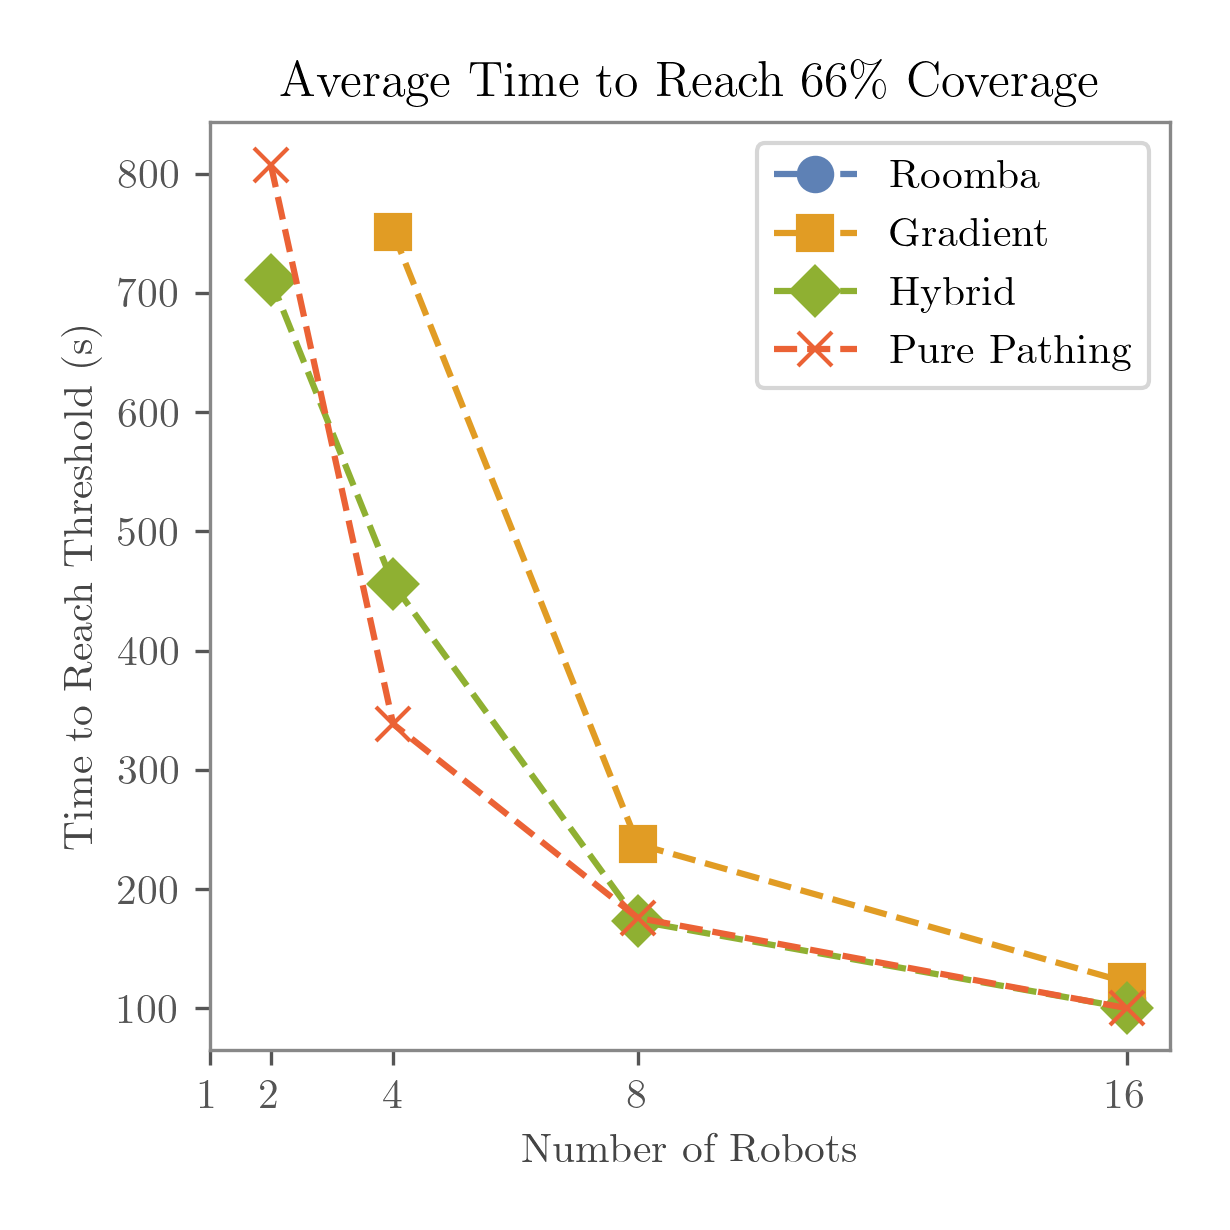
\includegraphics[width=\textwidth]{figures/plots/benchmarks/big-coverage-0.66-warehouse.png}
    \end{subfigure}
    \begin{subfigure}[b]{\w}
        \centering
        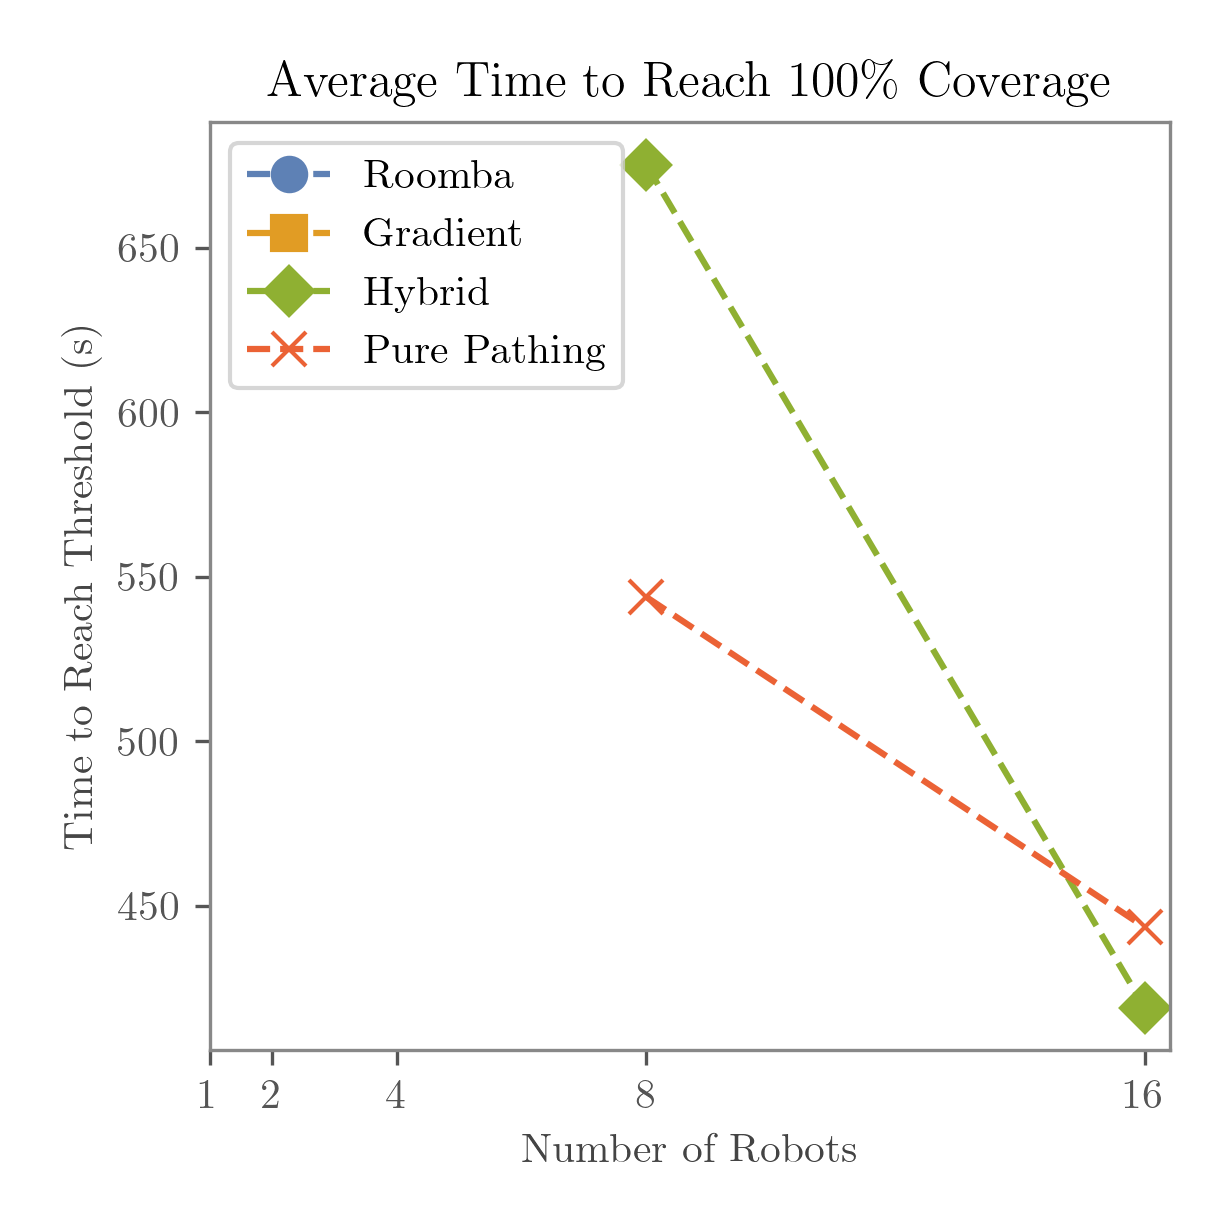
\includegraphics[width=\textwidth]{figures/plots/benchmarks/big-coverage-1.0-warehouse.png}
    \end{subfigure}
    \caption{Average time it takes the swarm to cover 33\%, 66\% and 100\% of the map in the Warehouse environment over 10 runs. Points are left out if the swarm did not reach these thresholds on average.}
    \label{fig:warehouse-threshold}
\end{figure}

\Cref{fig:depot-threshold} and \cref{fig:warehouse-threshold} show the average time required for the swarm to reach various coverage thresholds in the Depot and Warehouse environments, respectively, using different numbers of robots.

The results clearly indicate that the \textbf{Pure Pathing} and \textbf{Hybrid} behaviors are the most efficient in achieving higher coverage levels. This highlights the benefit of incorporating global map awareness and structured path planning into the search strategy.

In contrast, the \textbf{Roomba} algorithm demonstrates significantly reduced performance in the more complex Warehouse environment. Notably, it fails to surpass 33\% coverage within the trial duration, regardless of the number of robots. This suggests that simple obstacle-avoiding behaviors without global coordination are insufficient in environments with dense obstacle layouts and limited visibility.

\subsection{Computational Performance}
A critical aspect of the search algorithm's performance is computational requirement for running the behaviors.
\Cref{fig:computation-performance} shows the distribution of computation times per time step for each search algorithm, measured over six runs in the same environment. The data highlights key differences in computational cost and stability across behaviors.\\

As expected, the \textbf{Roomba} algorithm demonstrates the lowest and most consistent computation time due to its simplicity and lack of map processing. In contrast, the \textbf{Pure Pathing} algorithm performs efficiently on average but displays noticeable outliers. These spikes are caused by expensive operations --- such as costmap updates, frontier evaluation, and A* path planning --- which are not executed at every time step. This variability suggests a degree of computational instability that could pose challenges when deploying on resource-constrained platforms like microcontrollers.\\

The \textbf{Gradient} method, while computationally stable, exhibits the highest average computation time. This is due to the cost of recalculating the gradient field at every step, regardless of environmental changes. The \textbf{Hybrid} algorithm was expected to fall between Pure Pathing and Gradient in terms of computational load, which is consistent with the observed data. Its ability to switch between strategies allows it to balance responsiveness and efficiency without incurring the full cost of either method.

\begin{figure}[H]
    \begin{center}
        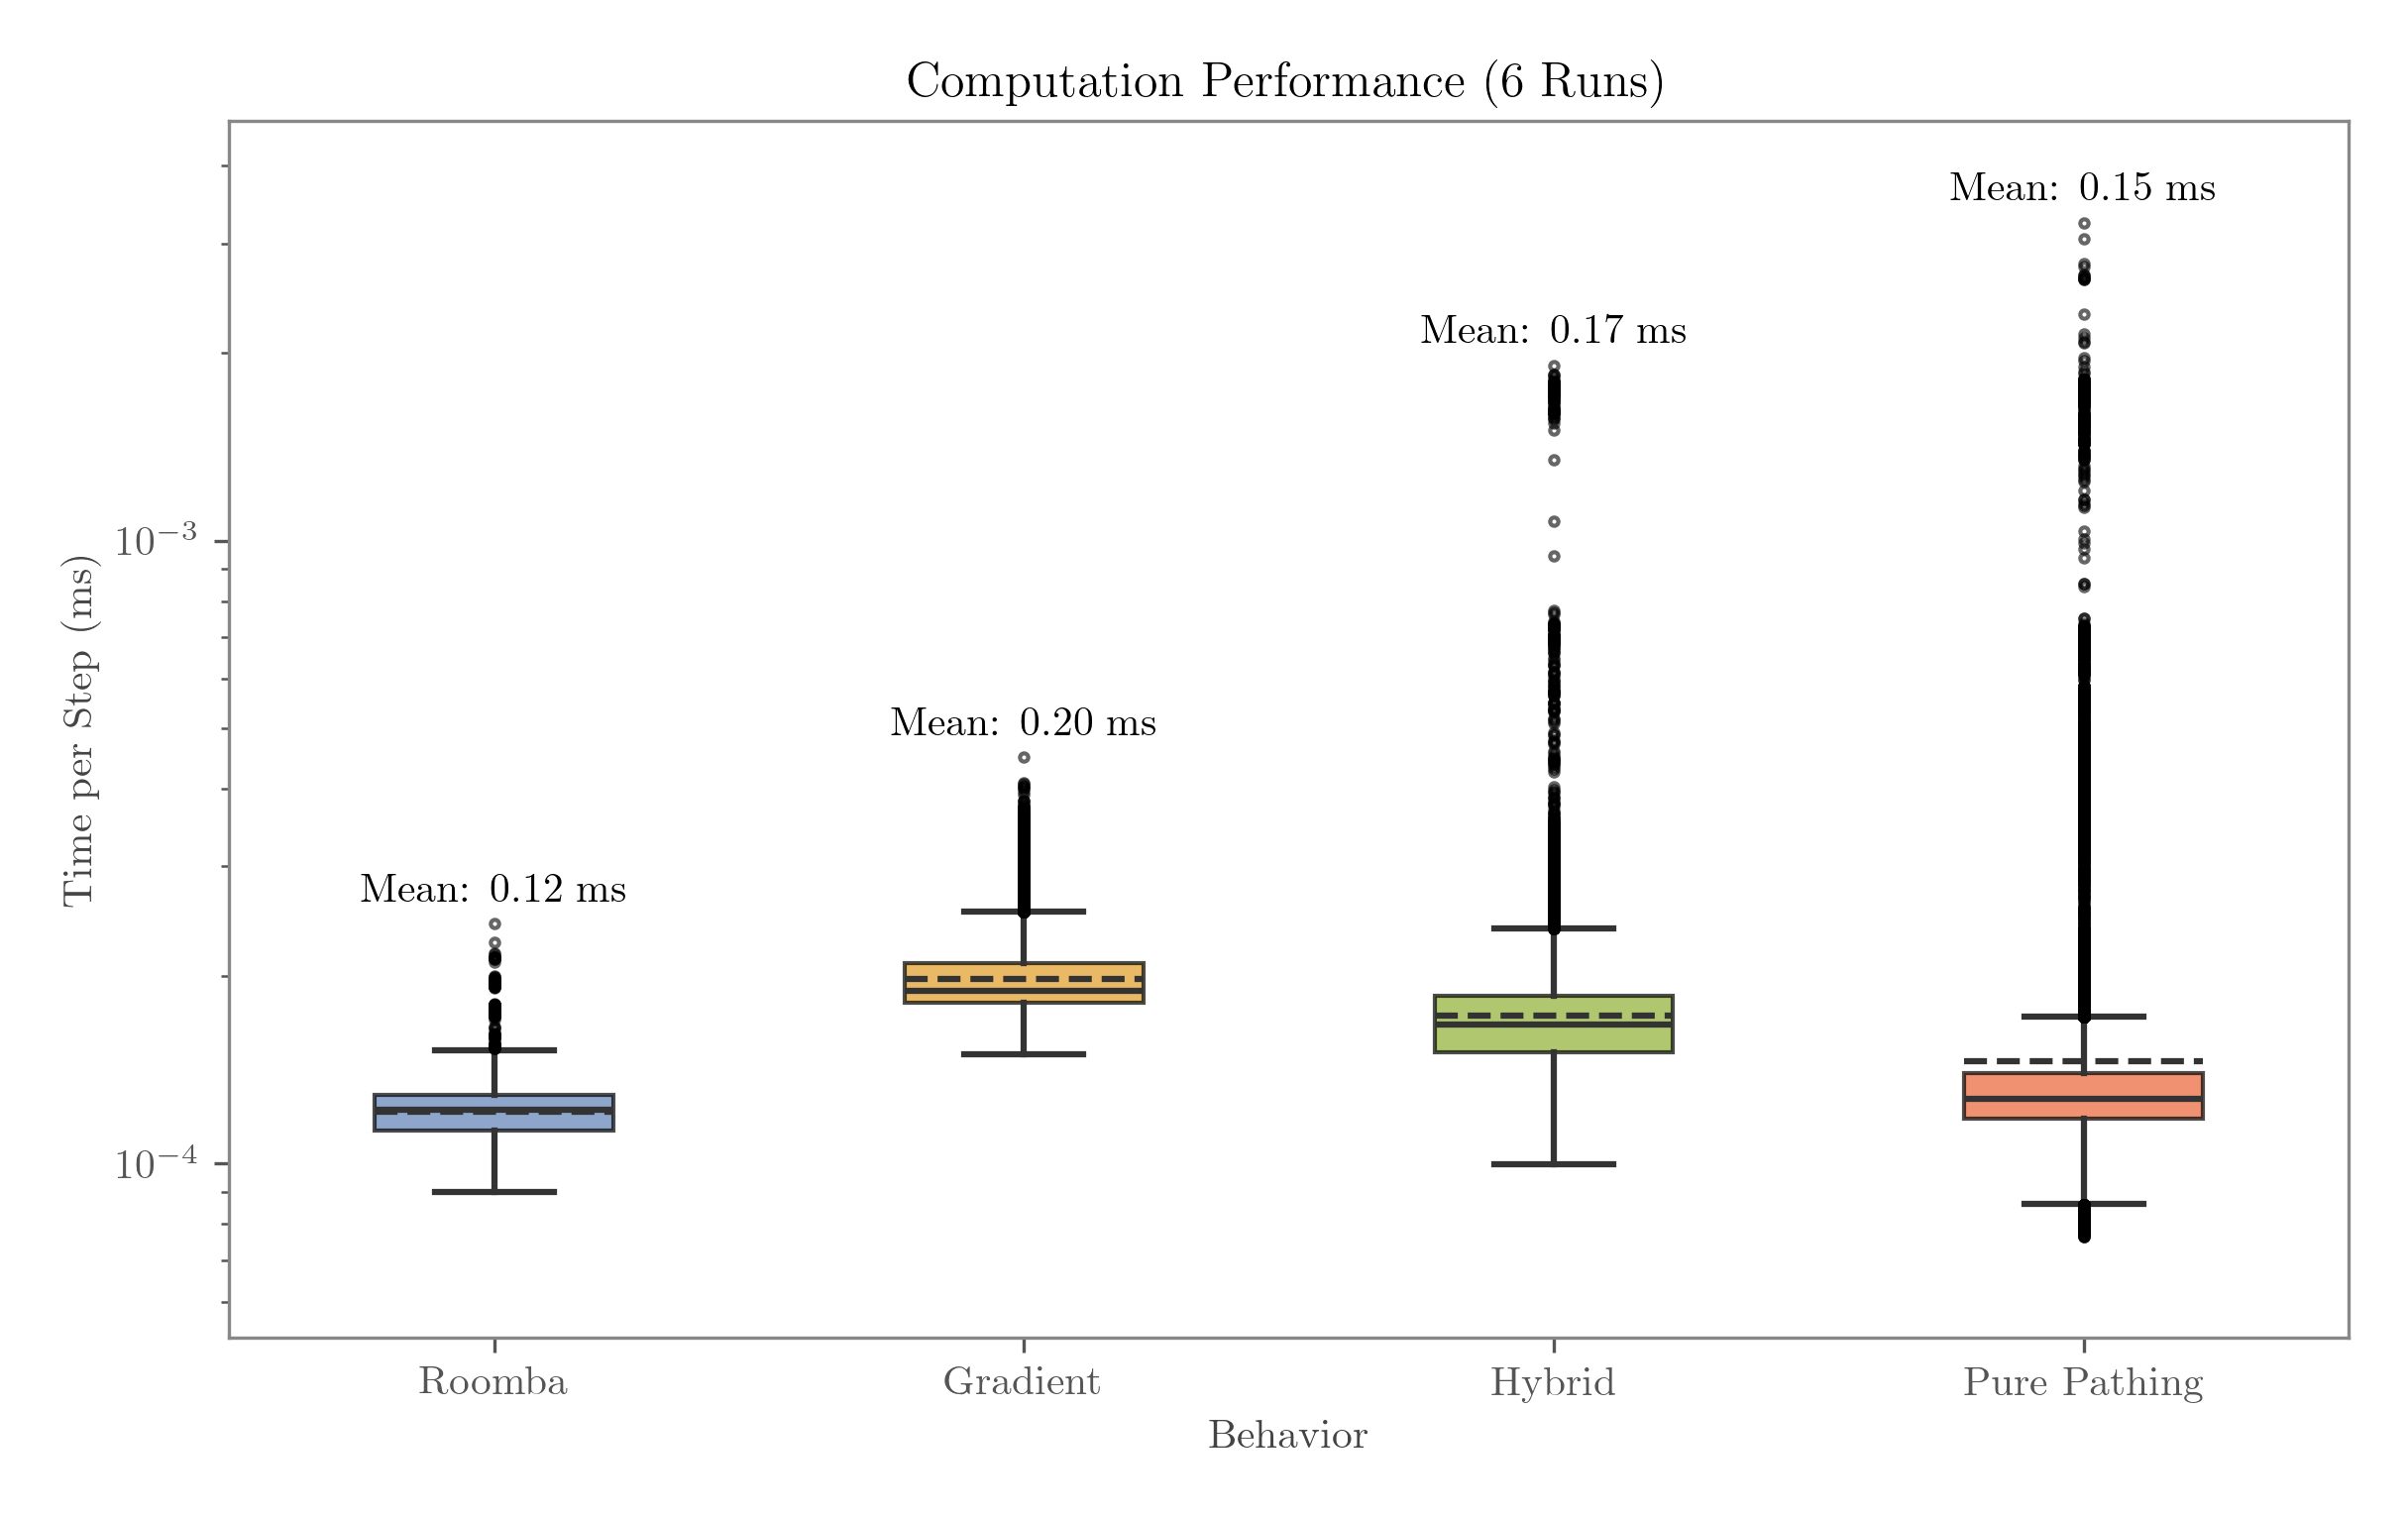
\includegraphics[width=0.95\textwidth]{./figures/plots/computation-performance-(6-runs).png}
    \end{center}
    \caption{Computation time for each search algorithm in the same map environment. Log scale is used for better visualization.}
    \label{fig:computation-performance}
\end{figure}

\subsection{Communication Load}
The messages transmitted during operation are updates to the search grid, which are sent whenever a robot’s internal search grid is modified. From these updates, other robots can synchronize their local search grids and infer the position of the robot that originated the message. Each message has a fixed size of 26 bytes. The \texttt{botbrain} library includes a configurable parameter that controls the broadcast frequency. The frequency is set to 10 Hz by default, which is one message every 100 ms, resulting in approximately 260 bytes/sec of outbound communication per robot. \\

A bandwidth of 260 bytes/sec negligible for most communicatino technologies considered for real-world deployment (see \cref{sub:communication-methods}), including Wi-Fi, Zigbee, and cellular. However, it may exceed practical limits for LoRa, particularly as the number of robots increases or in scenarios requiring higher message frequencies. If LoRa is to be considered for deployment, further message compression, reduced transmission frequency, or more aggressive filtering strategies would be necessary to meet the bandwidth constraints.

\subsection{Simulator Performance}
\label{sec:simulator-performance}
The performance and rapid iteration cycle offered by the \texttt{simple\_sim} simulator were key motivations for its development in this project. To quantify its efficiency, a simple benchmark was conducted by running both simulators headless (without a GUI) for 600 simulated seconds using the Roomba algorithm. Over 5 runs, Gazebo required 628 real-time seconds on average to complete the simulation, whereas \texttt{simple\_sim} completed the same task in an average of just 18 seconds. This substantial difference highlights the lightweight simulator’s superior computational performance.

The ability to run simulations significantly faster than real time is highly beneficial for development. It enables rapid experimentation, easier debugging, and efficient benchmarking of algorithmic changes—making \texttt{simple\_sim} a preferable tool during the design and testing phases.

\subsubsection{Gazebo Stability}
Benchmark data was collected with Python scripts which run both \texttt{simple\_sim} and Gazebo on the same environments automatically for a set of runs. Gazebo was, however, quite unreliable in its initialization which meant that Gazebo had to be supervised during benchmarking. This made it infeasible to run long trials multiple times with multiple behaviors. The following sections contain plots with data gathered using \texttt{simple\_sim} and would have taken days of supervised benchmarking to record using Gazebo.

